\documentclass{ieeeojies}
\usepackage{cite}
\usepackage{amsmath,amssymb,amsfonts}
\usepackage{algorithmic}
\usepackage{graphicx}
\usepackage{textcomp}
\usepackage{array}
\usepackage[table]{xcolor}
\usepackage{multirow}
\usepackage{multicol}
\usepackage{float}

\def\BibTeX{{\rm B\kern-.05em{\sc i\kern-.025em b}\kern-.08em
    T\kern-.1667em\lower.7ex\hbox{E}\kern-.125emX}}

\begin{document}
\title{Investigating the Efficacy of Statistical, Machine Learning, and Deep Learning Approaches in Steel Stock Price Prediction}

\author{\uppercase{Le Xuan Quynh}\authorrefmark{1},
\uppercase{Nguyen Thi Thuy Hang\authorrefmark{2}, and Truong Gia Man}\authorrefmark{3}}

\address[1]{Faculty of Information Systems, University of Information Technology, (e-mail: 21520430@gm.uit.edu.vn)}
\address[2]{Faculty of Information Systems, University of Information Technology, (e-mail: 21520822@gm.uit.edu.vn)}
\address[3]{Faculty of Information Systems, University of Information Technology, (e-mail: 21521115@gm.uit.edu.vn)}

\markboth
{Author \headeretal: Le Xuan Quynh, Nguyen Thi Thuy Hang and Truong Gia Man}
{Author \headeretal: Le Xuan Quynh, Nguyen Thi Thuy Hang and Truong Gia Man}

\begin{abstract}
This study investigates the efficacy of various algorithms for time series analysis on steel stock price data. We employ a dataset encompassing the prices of Hoa Phat Group, Hoa Sen Group, and Nam Kim Group from the Ho Chi Minh Stock Exchange (HOSE). The employed algorithms include Linear Regression, ARIMA, VARMA, Bagging with RNN, Recurrent Neural Networks (RNNs) with variants LSTM and GRU, and Residual Networks (ResNet). The performance of each algorithm is evaluated using metrics like Mean Absolute Error (MAE), Root Mean Squared Error (RMSE), and Mean Squared Error (MSE). This research aims to assess the effectiveness of these algorithms in capturing the inherent patterns within steel stock price time series data. The findings contribute to the development of time series analysis methodologies in the steel sector, providing valuable insights for further research on price prediction models.
\end{abstract}

\begin{keywords}
 Time series analysis, Steel stock prices, Statistical methods, Machine learning, Deep learning, LSTM, GRU, ResNet, ARIMA, VARMA, BaggingRNN.
\end{keywords}

\titlepgskip=-15pt

\maketitle

\section{Introduction}
\label{sec:introduction}

Accurate stock price forecasting is crucial for informed investment decisions in the steel sector. Investors and financial analysts rely on reliable predictions to identify potential investment opportunities and mitigate risks. However, stock price movements are inherently complex and influenced by a multitude of factors, making accurate forecasting a challenging task.

This study delves into the application of various statistical and machine learning algorithms for analyzing time series data in the context of steel stock price prediction. We aim to investigate the effectiveness of these algorithms in capturing the intricate patterns and trends within historical stock price data, thereby enhancing our understanding of time series analysis.

To achieve this objective, we employ a comprehensive dataset encompassing five years of historical stock trading data from different steel industry sectors. The input data spans from March 1, 2019, to June 1, 2024, providing a rich source of information for analyzing price patterns. Our primary focus lies in evaluating the performance of the models based on metrics like MAPE, MAE, RMSE, and predicting stock prices for the next 30, 60, and 90 days starting from June 1, 2024, to identify the trends in the time series.

The study employs a diverse range of algorithms, including Linear Regression models, VARMA (Vector Autoregressive Moving Average), ARIMA (Autoregressive Integrated Moving Average), BaggingRNN, Recurrent Neural Networks (RNNs) with their variants Long Short-Term Memory (LSTM) and Gated Recurrent Unit (GRU), and Residual Networks (ResNet). These algorithms represent a spectrum of statistical, machine learning, and deep learning techniques, each with its own strengths and limitations.

By evaluating the performance of these algorithms across different prediction horizons (30, 60, and 90 days), we aim to identify the most effective approaches for analyzing steel stock price time series data. The findings of this study will contribute to the advancement of time series analysis methodologies, providing valuable insights for financial analysts.

\section{Related Works}

In the article \cite{b1} focusing on Indonesia's export of oil and coal between 2002 and 2017, researchers employed the VARMA model to forecast production and quantity. Despite the initial non-stationarity of the dataset, confirmed by ACF and PACF analyses, they ensured data stationarity using the Augmented Dickey-Fuller unit root tests. Model selection was based on various information criteria, including AICC, HQC, AIC, and SBC. To enhance model accuracy, non-significant parameters such as those in AR-212, AR-221, and MA-121 were restricted. Furthermore, Granger causality tests indicated that oil exports were influenced solely by their own dynamics, not by coal exports.

This paper \cite{b2} highlights the strengths of GRUs in managing high volatility, capturing sharp price spikes, and addressing seasonality in electricity prices, demonstrating their superiority over traditional statistical models and other neural network structures. A significant takeaway from this study is the effectiveness of advanced RNNs architectures like GRUs in handling complex time series data. This observation leads to the consideration of optimizing training processes or integrating hybrid models to enhance efficiency without compromising accuracy. 

In the study \cite{b3} conducted by a group of students from Sogang University in Seoul, short-term load forecasting based on ResNet and LSTM was investigated. The research began by utilizing the ResNet model for load forecasting and then proposed a novel method for Short-Term Load Forecasting (STLF) by exploiting a combined ResNet/LSTM model. The strength of ResNet lies in image recognition, with the study focusing on detecting graphs within the data to produce results.

This paper \cite{b4} utilizes RNNs with LSTM to address the vanishing gradient problem. Trained on historical air quality and weather data from Taiwan, the model shows significant prediction accuracy improvements over traditional methods. It highlights the effective handling of time-series data and practical applications in environmental monitoring. Despite its success, the study points out the complexity and computational demands of LSTM models, suggesting the need for parameter tuning and model simplification. This underscores the importance of balancing model complexity with performance and provides valuable insights for future time-series forecasting research using RNNs.
\section{Materials}
\subsection{Dataset}
The primary objective of this research revolves around forecasting stock price movements within the steel sector. To achieve this goal, we utilize three distinct datasets sourced from reputable financial data providers. Specifically, the stock price data for Hoa Phat Group Joint Stock Company (HPG), Hoa Sen Group Joint Stock Company (HSG), and Nam Kim Steel Joint Stock Company (NKG) were collected from established stock market platforms. These datasets cover the period from March 1, 2019, to June 1, 2024, and encompass essential features pertinent to stock market analysis and prediction.
\begin{table}[H]
  \centering
  \caption{Describe attribute of dataset}
\begin{tabular}{|>{\columncolor{red!20}}c|c|c|c|}
    \hline
     \rowcolor{red!20} Arribute & Describe \\ \hline
     Date & Stock Trading Day \\ \hline
     Price & The closing price of the stock at a certein day (VND)\\ \hline
     Open & The opening price of the stock at a certain day (VND)\\ \hline
     High & Highest price of opening price (VND)\\ \hline
     Low & Lowest price of opening price (VND)\\ \hline
     Vol.& Number of transactions during the day\\ \hline
     Change \% & Percentage change in stock price from previous day's close\\ \hline
\end{tabular}
\end{table}
The purpose of the article is to predict the close prices, so only descriptive statistical data relating to column "Price" will be listed.
\subsection{Descriptive Statistics}
Perform descriptive statistics on the “Price” attribute across the datasets of steel sector companies' stock prices, including HPG, HSG, and NKG.
\begin{table}[H]
  \centering
  \caption{HPG, HSG, NKG’s Descriptive Statistics}
\begin{tabular}{|>{\columncolor{red!20}}c|c|c|c|}
    \hline
     \rowcolor{red!20} & HPG & HSG & NKG \\ \hline
     Count & 1313 & 1313 & 1313 \\ \hline
     Mean & 21,627 & 16,613 & 15,977\\ \hline
     Std & 9,431 & 9,498 & 10,366\\ \hline
     Min & 7,412 & 3,282 & 2,891\\ \hline
     25\% & 12,353 & 7,917 & 5,118\\ \hline
     50\% & 20,847 & 15,412 & 15,700\\ \hline
     75\% & 26,773 & 21,923 & 23,000\\ \hline
     Max & 43,895 & 41,541 & 44,965\\ \hline
     Mode & 18,909 & 14,663 & 4,008\\ \hline
     CV & 0.436 & 0.572 & 0.649\\ \hline
\end{tabular}
\end{table}
Based on Table 2, it is noted that the datasets are of equal size. The percentiles of the data also suggest a potential upward trend as values increase. Upon observing CV < 1, indicating that the standard deviation is smaller than the mean, the data exhibits moderate fluctuations. The steel industry data can be considered relatively stable due to its inherent stability.
\subsection{Visualization}
For time series data, use a Decomposition gragh to identify the data characteristics and utilize a Histogram to examine the data distribution.
\begin{figure}[H]
    \centering
    \begin{minipage}{0.23\textwidth}
    \centering
    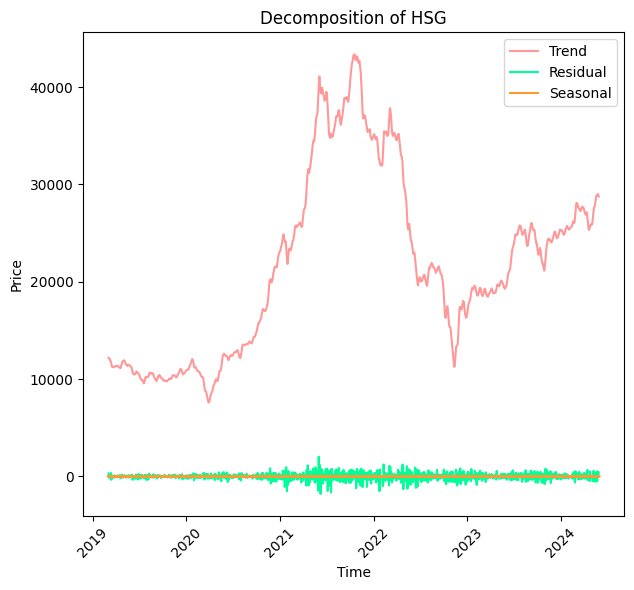
\includegraphics[width=1\textwidth]{bibliography/Figure/Decomposition_HPG.png}
    \caption{HPG stock price's decompostion}
    \label{fig:1}
    \end{minipage}
    \hfill
    \begin{minipage}{0.23\textwidth}
    \centering
    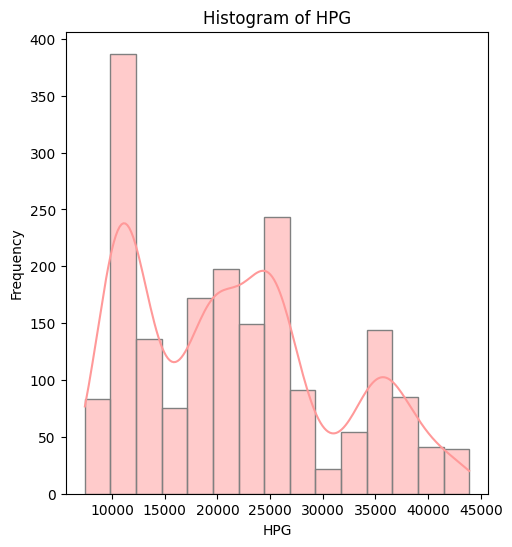
\includegraphics[width=1\textwidth]{bibliography/Figure/Histogram_HPG.png}
    \caption{HPG stock price's histogram}
    \label{fig:2}
    \end{minipage}
\end{figure}

\begin{figure}[H]
    \centering
    \begin{minipage}{0.23\textwidth}
    \centering
    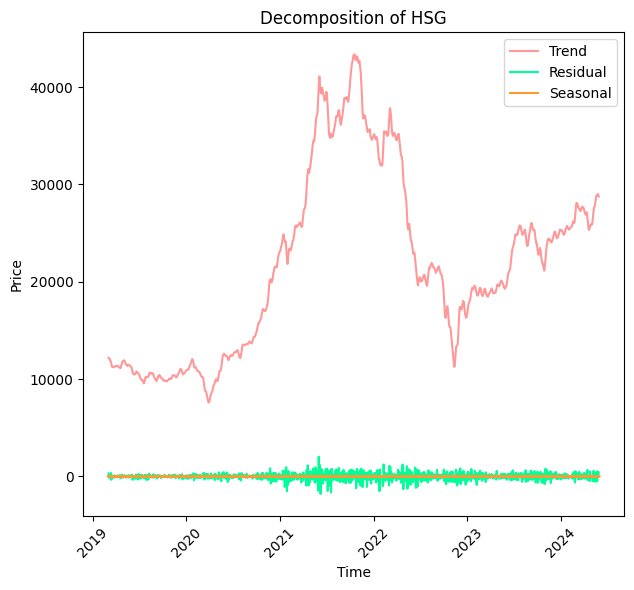
\includegraphics[width=1\textwidth]{bibliography/Figure/Decomposition_HSG.png}
    \caption{HSG stock price's decompostion}
    \label{fig:1}
    \end{minipage}
    \hfill
    \begin{minipage}{0.23\textwidth}
    \centering
    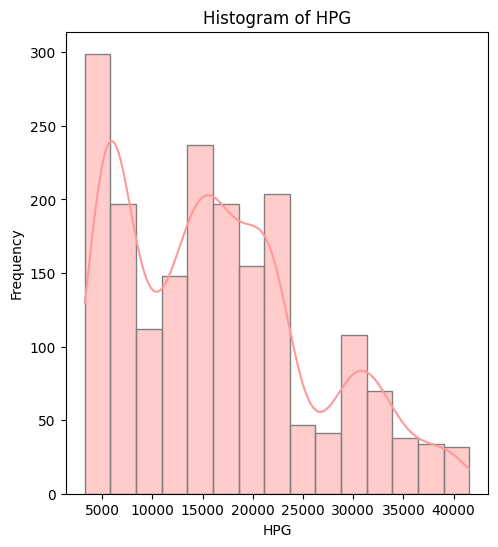
\includegraphics[width=1\textwidth]{bibliography/Figure/Histogram_HSG.png}
    \caption{HSG stock price's histogram}
    \label{fig:2}
    \end{minipage}
\end{figure}

\begin{figure}[H]
    \centering
    \begin{minipage}{0.23\textwidth}
    \centering
    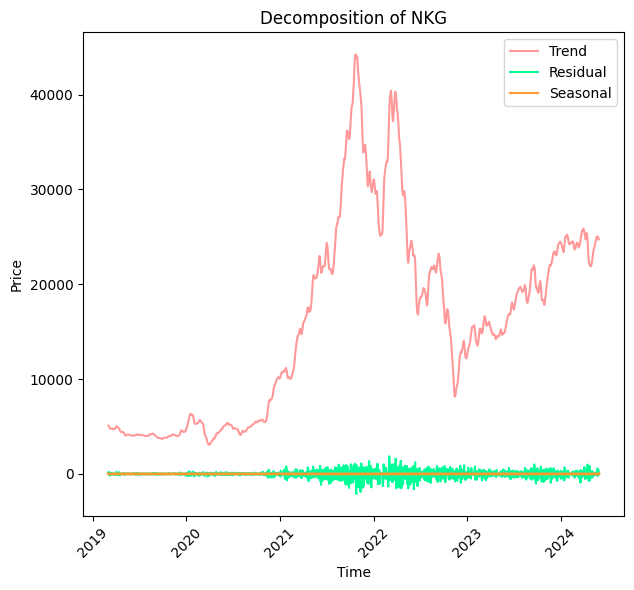
\includegraphics[width=1\textwidth]{bibliography/Figure/Decomposition_NKG.png}
    \caption{NKG stock price's decompostion}
    \label{fig:1}
    \end{minipage}
    \hfill
    \begin{minipage}{0.23\textwidth}
    \centering
    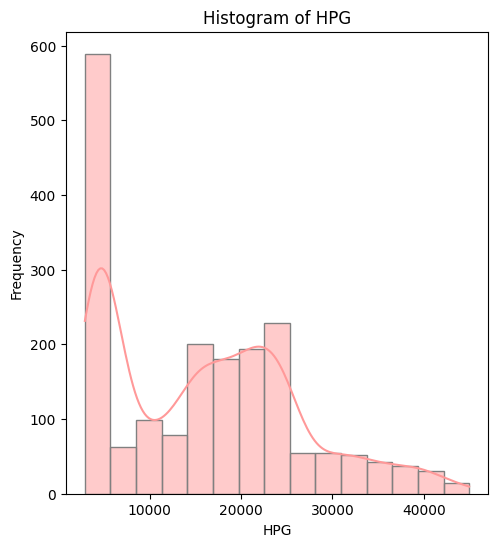
\includegraphics[width=1\textwidth]{bibliography/Figure/Histogram_NKG.png}
    \caption{NKG stock price's histogram}
    \label{fig:2}
    \end{minipage}
\end{figure}
Based on the Decomposition graph, it is observed that the dataset exhibits periods of rapid increase followed by sharp declines, then stabilizes at a moderate increase across all three datasets. Additionally, the dataset shows no seasonal pattern and has significant residual values. 

The Histogram reveals a skewed distribution towards lower values, indicating fewer occurrences of higher values in the dataset.
\subsection{Data Split Ratio}
In the context of a 5-year dataset, we considered three different splitting ratios: 80/20, 70/30, and 90/10. The 80/20 split offers a balanced approach with 80\% for training and 20\% for testing. The 70/30 split provides a larger testing set (30\%) for better generalization, while the 90/10 split focuses heavily on training (90\%) for a thorough model examination. The choice of ratio depends on dataset characteristics and machine learning goals, aiming for effective training and robust generalization.
\subsection{Evaluation Methods}
\textbf{Mean Percentage Absolute Error} (MAPE): is the average percentage error in a set of predicted values.\\
\[MAPE=\frac{100\%}{n}  \sum_{i=1}^{n} |y_i-\hat{y_i} |  = 1 \]\\
\textbf{Root Mean Squared Error} (RMSE): is the square root of average value of squared error in a set of predicted values.\\
\[RMSE=\sqrt{\sum_{i=1}^{n} \frac{(\hat{y_i}-y_i )^2}{n} }\]\\
\textbf{Mean Absolute Error} (MAE): is a metric used to measure
the average magnitude of errors between predicted and actual
values in a forecasting or regression model.\\
\[MAE = \frac{1}{n} \sum_{i=1}^n |y_i - \hat{y_i}|\]

Where: \\
	\indent\textbullet\ \(n\) is the number of observations in the dataset.\\
	\indent\textbullet\ \(y_i\)  is the true value.\\
	\indent\textbullet\ \(\hat{y_i}\) is the predicted value.
\section{Methodology}
\subsection{Linear Regression}
Regression analysis is a tool for building mathematical and statistical models that characterize relationships between a dependent variable and one or more independent, or explanatory, variables, all of which are numerical \cite{b5}. This statistical technique  is used to find an equation that best predicts the y variable as a linear function of the x variables \cite{b6}.
A multiple linear regression model \cite{b7} has the form: 
\[Y=\beta_0+\beta_1X_1+\beta_2X_2+\cdots+\beta_kX_k+\varepsilon\]
Where:\\
	\indent\textbullet\ Y is the dependent variable (Target Variable).\\
	\indent\textbullet\ \(X_1, X_2, \ldots, X_k\) are the independent (explanatory) variables.\\
	\indent\textbullet\ \(\beta_0\) is the intercept term.\\
	\indent\textbullet\ \(\beta_1,..., \beta_k\) are the regression coefficients for the independent variables.\\
	\indent\textbullet\ \(\varepsilon\) is the error term.
\subsection{ARIMA}
In 1970, Box and Jenkins introduced the ARIMA (Autoregressive Integrated Moving Average) model \cite{b8}. It is also known as the Box-Jenkins methodology, which is based on the autoregressive (AR) and moving average (MA) models. ARIMA is a quantitative forecasting model where the future value of the forecast variable depends on the historical trend of that variable\cite{b9}.
ARIMA is a popular model commonly used for time series forecasting. It has three components: AR, MA, and I.
\subsubsection{Autoregressive (AR)}
The Autoregressive (AR) component consists of a set of lags of the current variable. The lag of order \(p\) is essentially the value shifted back \(p\) time steps of the series. The length of the lag, whether long or short in this AR process, will depend on the lag parameter\(p\)\cite{b10}. Specifically, the \(\mathbf {AR}(p)\) process of the series \(\mathbf x_t\)is represented as the following formula:
\[\mathbf {AR}(p) = \phi_1 y_{t-1} + \phi_2 y_{t-2} + \dots + \phi_p y_{t-p} + \varepsilon_t\]
\subsubsection{Moving Average (MA)}
The Moving Average process adjusts the mean of a time series, resembling white noise (error term) due to its stationarity assumption\cite{b9}. A series \(\epsilon_t\) is called white noise if it satisfies the conditions of zero expectation, zero correlation at different lags, and constant variance of the error term\cite{b10}. It is represented by the following system of equations:
\begin{align*}
\mathbb{E}(\varepsilon_t) &= 0 \\
\sigma(\varepsilon_t) &= \alpha\\
\text{corr}(\varepsilon_t, \varepsilon_{t-s}) &= 0, \quad \forall s \leq t
\end{align*}
The Moving Average process can be represented by white noise as follows:
$$MA(q) =  + \theta_1 \varepsilon_{t-1} + \dots + \theta_q\varepsilon_{t-q}$$
\subsubsection{Integrated (I)}
Differencing (integration) creates stationary time series (constant statistics) by removing trends. The number of times we difference the data \(d\) is the ARIMA integration order\cite{b10}. The process of differencing a series of order \(d\) is performed as follows:\\
	\indent\textbullet\ First-order differencing: 
        $$I(1) = \Delta(x_t) = x_t -x_{t-1}$$
        \indent\textbullet\ Differencing of order \(d\):
        $$I(d) = \Delta^d(x_t) = \Delta(\Delta(\dots\Delta(x_t)))$$
The \(\mathbf {ARIMA(p,d,q)}\) regression equation can be represented as:
\begin{equation}
\begin{split}
\Delta(x_t) &= \phi_1\Delta(x_{t-1}) + \phi_2\Delta(x_{t-2}) + \dots + \phi_p\Delta(x_{t-p}) \\
&+ \theta_1 \varepsilon_{t-1} + \theta_2 \varepsilon_{t-2} + \dots + \theta_q\varepsilon_{t-q}
\end{split}
\end{equation}
Where \(\Delta(x_t)\) is the differenced value of order \(\mathbf d\) of the series and \(\epsilon_t\) is the white noise error term.
\subsection{VARMA}
VARMA modeling is a tool for building mathematical and statistical models that characterize relationships between multiple time series variables, which are numerical and evolve over time and produce linear forecasting \cite{b11}. This statistical technique is used to find a set of equations that best predict a vector of variables as a function of their past values and past shocks (unexpected events) \cite{b12}. VARMA model \cite{b13} has the form:
\begin{equation}
\begin{split}
\mathbf{Y}_t &= \mathbf{\Phi}_1 \mathbf{Y}_{t-1} + \mathbf{\Phi}_2 \mathbf{Y}_{t-2} + \dots + \mathbf{\Phi}_p \mathbf{Y}_{t-p} \\
&\quad + \mathbf{\epsilon}_t + \mathbf{\Theta}_1 \mathbf{\epsilon}_{t-1} + \mathbf{\Theta}_2 \mathbf{\epsilon}_{t-2} + \dots + \mathbf{\Theta}_q \mathbf{\epsilon}_{t-q}
\end{split}
\end{equation}
\\
Where: \\ 
         \indent\textbullet\ \(\mathbf{Y}_t\)\ is a vector containing the values of the k variables at time t. \\
         \indent\textbullet\ \(\mathbf{\Phi}_1,\,\mathbf{\Phi}_2, \ldots, \mathbf{\Phi}_n\)\ are matrices of coefficients that capture the autoregressive (AR) relationships, showing how past values of the variables influence their current values. \\
         \indent\textbullet\ \textbf{p} is the order of the AR component (the number of past time steps included). \\
         \indent\textbullet\ \({\epsilon}(t)\) is  a vector of error terms (shocks or innovations) at time \textit{t}. \\
         \indent\textbullet\ \({\Theta}_1, {\Theta}_2, \ldots ,{\Theta}_q\) are matrices of coefficients that capture the moving average (MA) relationships, showing how past shocks influence the current values of the variables. \\
         \indent\textbullet\ \textbf{q} is the order of the MA components (the number of past shocks included). 
\subsection{Bagging RNN-GRU}
Bagging, an abbreviation for Bootstrap Aggregating, is a machine learning ensemble strategy for enhancing the reliability and precision of predictive models. It entails generating numerous subsets of the training data by employing random sampling with replacement. These subsets train multiple base learners, such as decision trees, neural networks, or other models\cite{b14}.

Bagging is particularly effective in reducing variance and preventing overfitting, as each model in the ensemble can capture different aspects of the data's variability.

When applying Bagging to Recurrent Neural Networks (RNNs) and Gated recurrent units (GRUs), the technique leverages the strengths of RNNs and GRUs in modeling sequential data. The process involves creating new datasets using the bootstrap technique and training N models. The predictions from these models are aggregated through voting (for classification tasks) or averaging (for regression tasks). 
This hybrid methodology of Bagging and RNNs-GRUs, termed BaggingRNN-GRU, is advantageous in tasks such as time series forecasting, natural language processing, and any domain where sequential data is prevalent.

\subsection{RNN}
Recurrent Neural Networks (RNNs) are deep learning models that can be utilized for time series analysis, with recurrent connections that allow them to retain information from previous time steps\cite{b10}.The below equation represent a RNN cell:
\[h_t = g(W_{xh}x_t + W_{hh}h_{h-1} + c) \]
Where: \\ 
        \indent\textbullet\ \(\mathbf h_{t}\): The hidden state at time step t\\
        \indent\textbullet\ \(\mathbf g\): The activation function, commonly a non-linear function like tanh or ReLU\\
        \indent\textbullet\ \(\mathbf x_t\)\: The input at the current time step t\\
        \indent\textbullet\ \(\mathbf h_{t-1}\)\: The hidden state from the previous time step  \(\mathbf t-1\)\\
        \indent\textbullet\ \(\mathbf c \)\: The bias term\\
        \indent\textbullet\ \(\mathbf W_{xh}\)\: The weight matrix for the input \(\mathbf x_t\) \\
        \indent\textbullet\ \(\mathbf W_{hh}\): The weight matrix for the input \(\mathbf h_{t-1}\)\\

The weights of the RNN are updated through the Backpropagation Through Time (BPTT) algorithm. BPTT is an extension of the backpropagation algorithm used for training feedforward neural networks, adapted to handle the temporal nature of RNNs. During BPTT, the network is unrolled in time, and gradients are computed for each time step. The gradients are then propagated backward through time to update the weights.

RNNs can be categorized based on the configuration of inputs and outputs: one to one; one to many; many to one and many to many\cite{b16}
The choice of activation function g significantly affects the performance and behavior of the RNN: Tanh, ReLU, Sigmoid. The architecture of the RNN and the choice of hyperparameters (like the activation function) play crucial roles in their performance\cite{b17}
\subsection{LSTM}

Long Short-Term Memory (LSTM) networks have emerged as a prominent architecture in deep learning, particularly for tasks involving sequential data \cite{b18}. LSTMs address the vanishing gradient problem that plagues traditional Recurrent Neural Networks (RNNs), enabling them to effectively capture long-term dependencies \cite{b19}.

The fundamental building block of an LSTM is the memory cell, which maintains its state over time \cite{b18}. This cell is equipped with three gates: the forget gate, input gate, and output gate. These gates regulate the flow of information into and out of the cell, allowing the LSTM to selectively retain or discard information \cite{b19}. The forget gate determines which information from the previous state to forget, the input gate controls what new information to add to the cell state, and the output gate decides what information to output based on the cell state and current input \cite{b18}.
\begin{align*}
  \text{Forget Gate:} \quad & f_t = \sigma(W_f [h_{t-1}, x_t] + b_f) \\
  \text{Input Gate:} \quad & i_t = \sigma(W_i [h_{t-1}, x_t] + b_i) \\
  & \tilde{C}_t = \tanh(W_C [h_{t-1}, x_t] + b_C) \\
  \text{Output Gate:} \quad & o_t = \sigma(W_o [h_{t-1}, x_t] + b_o) \\
  \text{Cell State:} \quad & C_t = f_t * C_{t-1} + i_t * \tilde{C}_t \\
  \text{Hidden State:} \quad & h_t = o_t * \tanh(C_t)
\end{align*} 
Where: \\
         \indent\textbullet\ \textbf{\(\mathbf{x}_t\)}: The input vector at time step (t). \\
         \indent\textbullet\ \textbf{\(\mathbf{h}_t\)}: The hidden state (output) at time step (t). \\
         \indent\textbullet\ \textbf{\(\mathbf{C}_t\)}: The cell state (internal memory) at time step (t). \\
         \indent\textbullet\ \textbf{\(\mathbf{W}_f,\, \mathbf{W}_i,\, \mathbf{W}_C,\ \mathbf{W}_o,\)}: Weight matrices for the forget, input, cell, and output gates, respectively. \\ 
         \indent\textbullet\ \textbf{\(\mathbf{b}_f,\, \mathbf{b}_i,\, \mathbf{b}_C,\ \mathbf{b}_o,\)}: Bias vectors for the forget, input, cell, and output gates, respectively. \\
         \indent\textbullet\ \(\sigma\): The sigmoid activation function, which squashes values between 0 and 1, representing how much information to let through the gate. \\ 
         \indent\textbullet\ \(\tanh\): The hyperbolic tangent activation function, which squashes value between -1 and 1, used to regulate the cell state. \\ \\
Interpretations \cite{b18}: \\
         \indent\textbullet\ \textbf{Forget Gate} (\(\mathbf{f}_t\)): 
         Determines what information to keep or discard from the previous cell state \(\mathbf{C}_{t-1}\). \\
         \indent\textbullet\ \textbf{Input Gate} (\(\mathbf{i}_t\)): Controls how much of the new information from the current input \(\mathbf{x}_t\) and previous hidden state \(\mathbf{h}_{t-1}\) should be added to the cell state. \\
         \indent\textbullet\ \textbf{Cell State} (\(\mathbf{C}_t\)): Maintains the LSTM's long-term memory, updated by combining the filtered old cell state and new information. \\
         \indent\textbullet\ \textbf{Output Gate} (\(\mathbf{o}_t\)): Controls how much of the cell state is used to update the hidden state \(\mathbf{h}_t\), which is the output of the LSTM cell. \
 \subsection{GRU}
The Gated Recurrent Unit (GRU) stands as an improvement upon the Long Short-Term Memory (LSTM) network\cite{b20} . This advancement is primarily attributed to its gating mechanism, which controls how past information ($h_{t-1}$) and current input ($x_t$) are incorporated into the model's hidden state ($h_t$). The core difference lies in GRU cells combining the forget gate and input gate of LSTMs into a single update gate ($z_t$).
The mathematical equations governing the relationship between input and output within the GRU cell are presented as follows \cite{b20}:
\begin{align*}
\text{Update gate:} \quad & z_t = \sigma(W_z \cdot [h_{t-1}, x_t]) \\
\text{Reset gate:} \quad & r_t = \sigma(W_r \cdot [h_{t-1}, x_t]) \\
\text{Candidate hidden state} \quad & h_t \tilde{} = \tanh(W \cdot [r_t \odot h_{t-1}, x_t]) \\
\text{Hidden state:} \quad & h_t = (1 - z_t) \odot h_{t-1} + z_t \odot h_t \tilde{} \\
\end{align*}

Within these equations, $\sigma(.)$ represents the sigmoid function, $\tanh(.)$ signifies the hyperbolic tangent function, $W_z$ and $W_r$ denote the weights associated with the update and reset gates, respectively, $\odot$ denotes the element-wise product, and $h_{t-1}$ and $x_t$ symbolize the previous hidden state and current input. The reset gate is responsible for capturing short-term dependencies within the sequence data, while the update gate plays a crucial role in learning long-term dependencies \cite{b20}.
\subsection{ResNet}
ResNet (Residual Neural Network) extends the depth of neural networks by introducing shortcut connections within residual blocks, enabling the gradient flow to propagate directly through the bottom layers. This has led to remarkable performance in object recognition and other vision-related tasks {\cite{b21}}. Intrigued by the potential of deep neural networks for time series data analysis, we explore the ResNet architecture. While overfitting is a concern given the relatively small and variant-deprived UCR datasets, employing a deeper model and examining its strengths and weaknesses remains a valuable exercise. To construct each residual block, we reuse the convolutional blocks from Equation 2. Let Blockk denote a convolutional block with filter size k, and the residual block is formalized as:
\begin{align*}
h_1 &= \text{Block}_k^1(x) \\
h_2 &= \text{Block}_k^2(h_1) \\
h_3 &= \text{Block}_k^3(h_2) \\
y &= h_3 + x \\
\hat{y} &= \text{ReLU}(y) \quad (3)
\end{align*}
Where the number of filters in each convolutional block is denoted by ki = {64, 128, 128}. The final ResNet stacks three residual blocks followed by a global average pooling layer and a softmax layer. For this task, we employ a kernel size of [7, 5, 3] for the three convolutional layers within each residual block.
\section{Result}
This section describes an experiment that evaluates the performance of eight algorithms applied to three datasets. 

For the statistical algorithms, Linear Regression, ARIMA, and VARIMA all take the input data directly. However, for VARMA, which is based on other time series, a correlation matrix is used to find suitable dependencies to use as additional time series.

For machine learning and deep learning algorithms, the data needs to be normalized into a matrix format before creating the model and feeding the data into the neural network. For the ResNet model, we need to create a dataset in a format that is compatible with PyTorch.

For deep learning algorithms, Adam is additionally used to optimize the model.
\subsection{HPG Dataset} 
\begin{table}[H]
    \centering
    \begin{tabular}{|c|c|c|c|c|}
         \hline
         \multicolumn{5}{|c|}{\textbf{HPG Dataset's Evaluation}}\\
         \hline
         \centering Model & Training:Testing & RMSE & MAPE (\%) & MAE\\
         \hline
         \multirow{2}{*}{LN} & 7:3 & 20348.75 & 188.09 & 20262.29 \\ & 8:2 & 11276.39 & 106.56 & 11243.7 \\ & \textbf{9:1} & \textbf{5717.21} & \textbf{52.58} & \textbf{5623.63}\\
         \hline
         \multirow{2}{*}{ARIMA} & 7:3& 7994.3 & 31.49 & 3261.17 \\ & 8:2& 2008.16&17.36&1885.4 \\ & \textbf{9:1} & \textbf{1323,93} & \textbf{10.01} & \textbf{1132.28}\\
         \hline
         \multirow{2}{*}{VARMA} & 7:3	& 7994.3 & 30.52 & 7232.81 \\ & 8:2 & 4862.47 & 17.13 & 4406.31 \\ & \textbf{9:1} & \textbf{2755.15}  & \textbf{8.35} & \textbf{2270.43}\\
         \hline

        \multirow{2}{*}{Bagging} & 7:3	& 320.17 & 2.49 & 264.12 \\& 8:2 & 214.5 & 1.51 & 160.19 \\ {RNN-GRU}& \textbf{9:1} & \textbf{218.06}  & \textbf{1.48} & \textbf{159.42}\\
         \hline
         
         \multirow{2}{*}{RNN} & 7:3	& 378.74 & 0.03 & 301.27 \\ & 8:2 & 240.22 & 1.75 & 185.46 \\ & \textbf{9:1} & \textbf{220.91} & \textbf{1.57} & \textbf{168.5}\\
         \hline
         \multirow{2}{*}{GRU} & 7:3 & 352.62&2.66 & 283.82 \\ & \textbf{8:2} &	\textbf{210.26} & \textbf{1.43} & \textbf{150.74} \\ & 9:1 &228.11	&1.64&176.59\\
         \hline
         \multirow{2}{*}{LSTM} & 7:3 & 1,916.3 & 17.283 & 1,807.287 \\ & 8:2 & 524.026 & 4.138  & 450.317 \\ & \textbf{9:1} &  	\textbf{312.454} &	\textbf{2.258} &\textbf{247.481} \\
         \hline
         \multirow{2}{*}{ResNet} & \textbf{7:3} & 3201.02 & \textbf{24.98} & \textbf{2499.34} \\ & 8:2 & 2977.36 &  27.29 &  2910.95 \\ & 9:1 & \textbf{2873.29} &  26.48 &  2862.73 \\
         \hline
    \end{tabular}
    \caption{HPG Dataset's Evaluation}
    \label{vcbresult}
\end{table}
For the HPG Stock data, it was observed that based on the evaluation metrics, most of the models achieved their best results on the 90/10 test set (except for ResNet and GRU). For the RNN algorithms, GRU and BaggingRNN-GRU with the three splitting methods gave good results, not too different from each other, indicating that the data has diverse fluctuations.
\begin{figure}[H]
  \centering
  \begin{minipage}{0.8\linewidth}
    \centering
    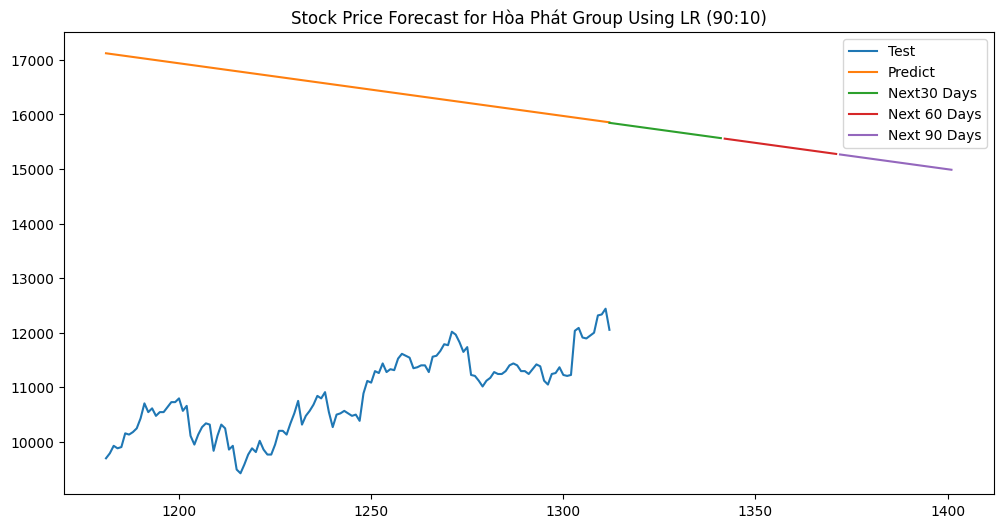
\includegraphics[width=\linewidth]{bibliography/LN_HPG_90-10.png}
    \caption{Linear Regression model's result with 9:1 splitting proportion}
    \label{fig8}
  \end{minipage}
\end{figure}
\begin{figure}[H]
  \centering
  \begin{minipage}{0.8\linewidth}
    \centering
    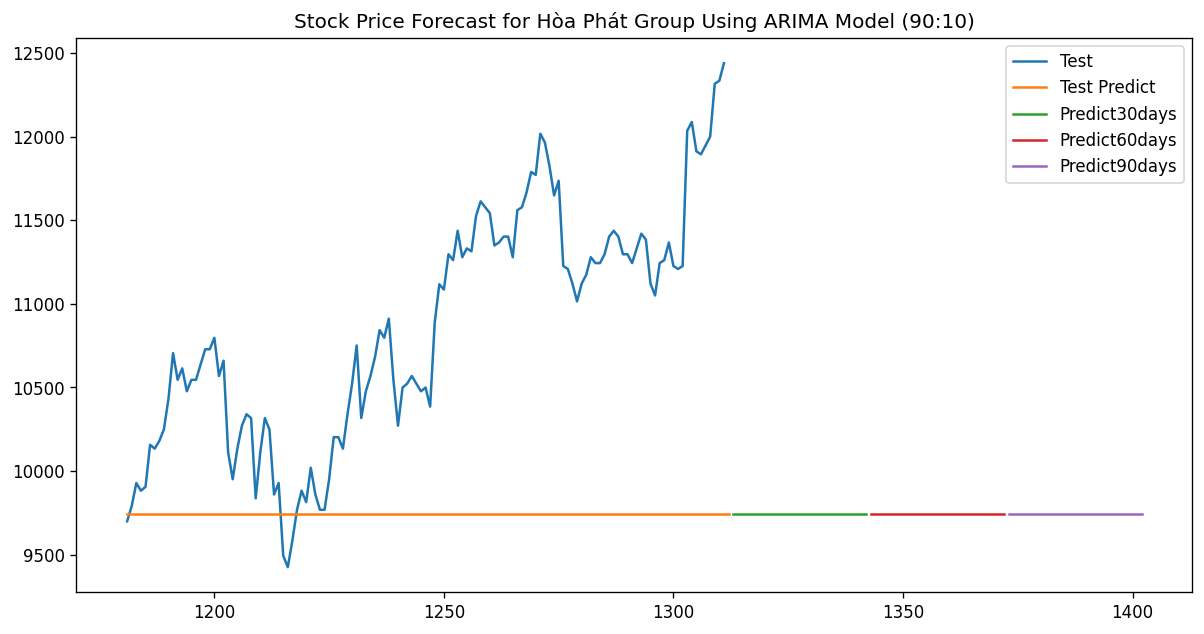
\includegraphics[width=\linewidth]{bibliography/ARIMA_HPG_90-10.png}
    \caption{ARIMA model's result with 9:1 splitting proportion}
    \label{fig9}
  \end{minipage}
\end{figure}
\begin{figure}[H]
  \centering
  \begin{minipage}{0.8\linewidth}
    \centering
    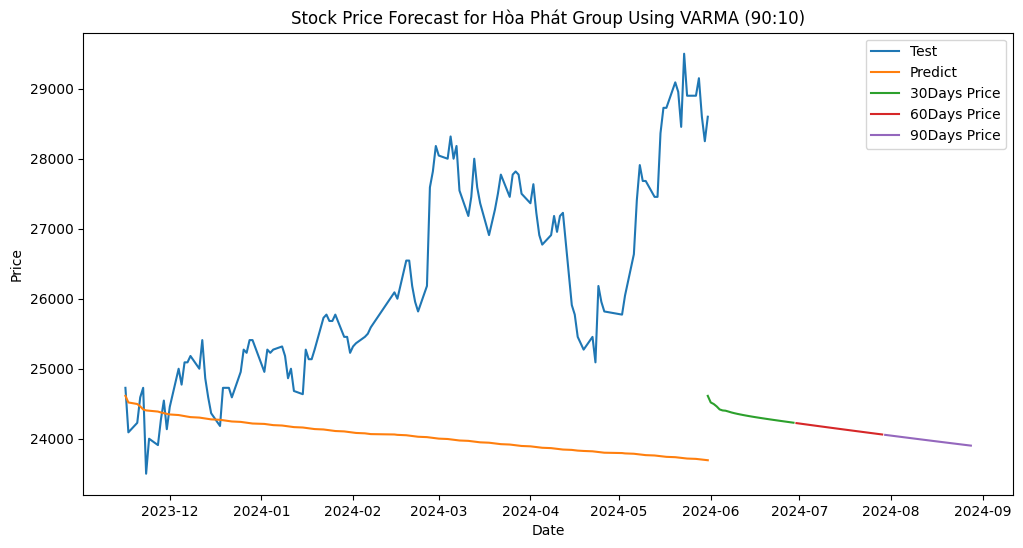
\includegraphics[width=\linewidth]{bibliography/VARMA_HPG_90-10.png}
    \caption{VARMA model's result with 9:1 splitting proportion}
    \label{fig10}
  \end{minipage}
\end{figure}
\begin{figure}[H]
  \centering
  \begin{minipage}{0.8\linewidth}
    \centering
    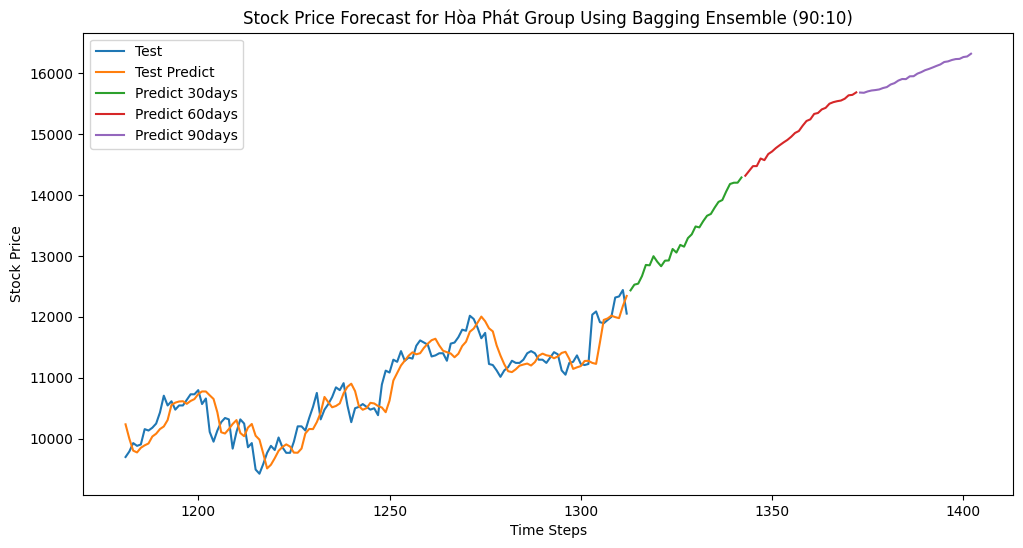
\includegraphics[width=\linewidth]{bibliography/Bagging_HPG.png}
    \caption{BaggingRNN-GRU model's result with 9:1 splitting proportion}
    \label{fig11}
  \end{minipage}
\end{figure}
\begin{figure}[H]
  \centering
  \begin{minipage}{0.8\linewidth}
    \centering
    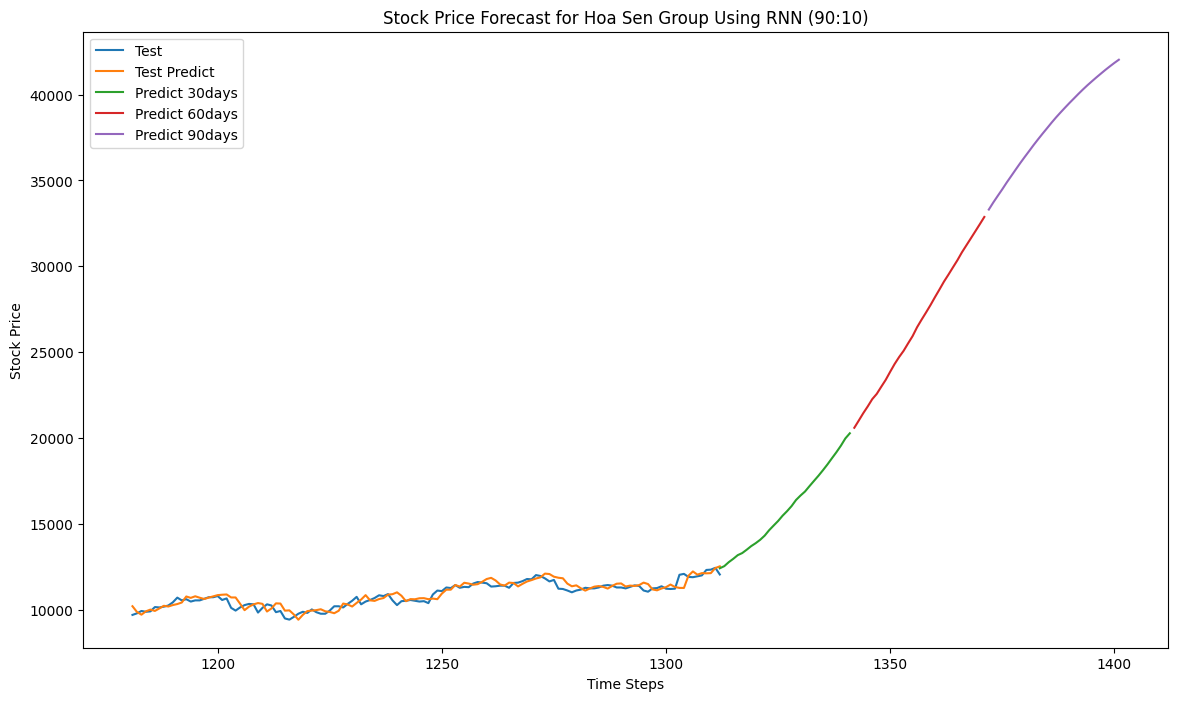
\includegraphics[width=\linewidth]{bibliography/RNN_HPG.png}
    \caption{RNN model's result with 9:1 splitting proportion}
    \label{fig12}
  \end{minipage}
\end{figure}
\begin{figure}[H]
  \centering
  \begin{minipage}{0.8\linewidth}
    \centering
    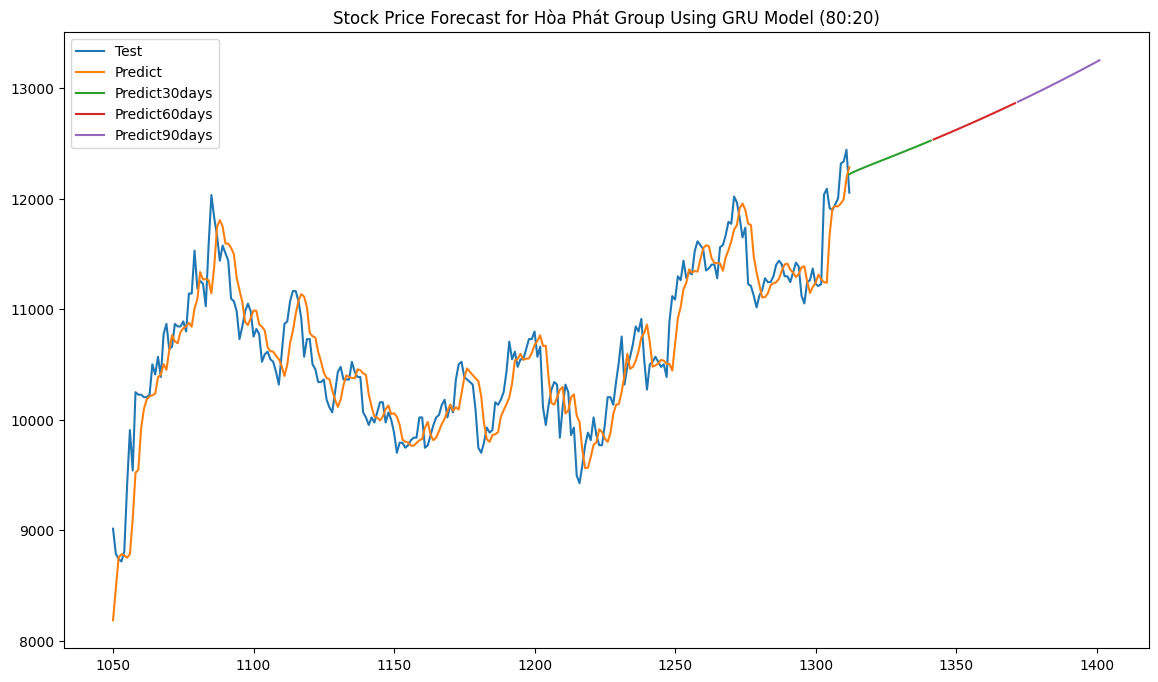
\includegraphics[width=\linewidth]{bibliography/GRU_HPG_80-20.png}
    \caption{GRU model's result with 8:2 splitting proportion}
    \label{fig13}
  \end{minipage}
\end{figure}
\begin{figure}[H]
  \centering
  \begin{minipage}{0.8\linewidth}
    \centering
    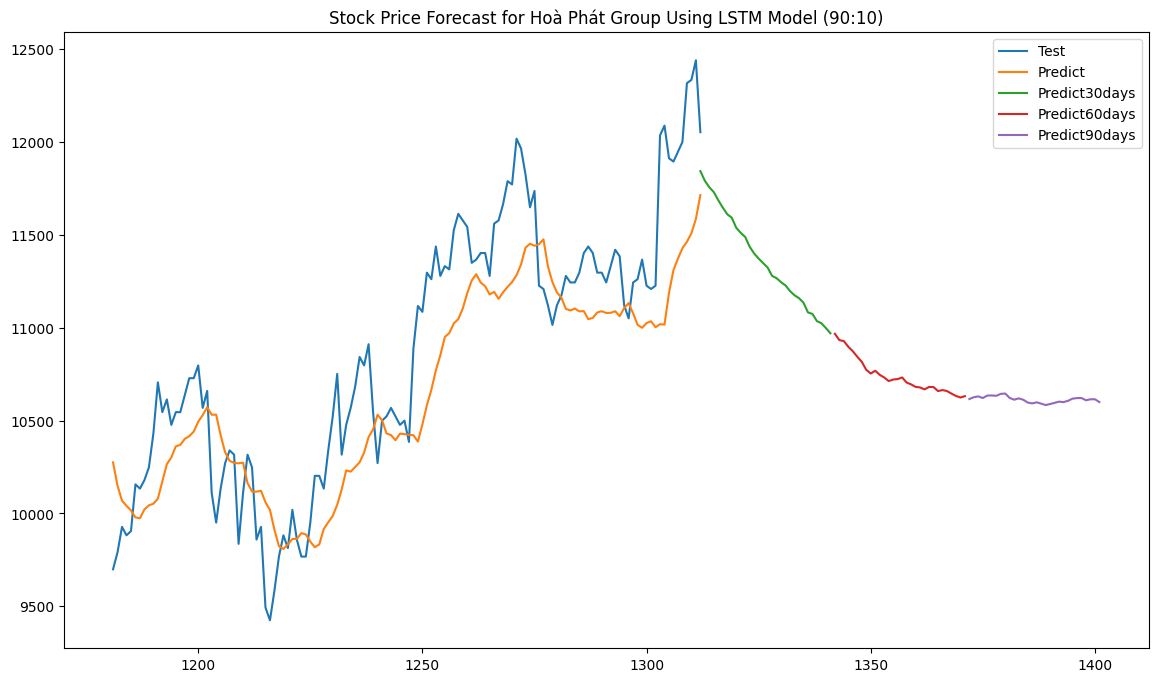
\includegraphics[width=\linewidth]{bibliography/LSTM_HPG_90-10.png}
    \caption{LSTM model's result with 9:1 splitting proportion}
    \label{fig14}
  \end{minipage}
\end{figure}
\begin{figure}[H]
  \centering
  \begin{minipage}{0.8\linewidth}
    \centering    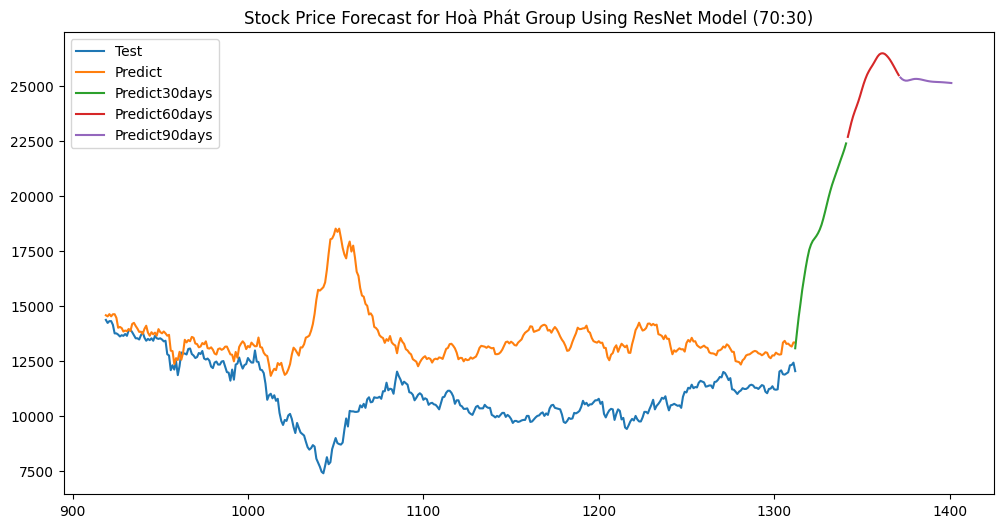
\includegraphics[width=\linewidth]{bibliography/ResNet_HPG_70-30.png}
    \caption{ResNet model's result with 7:3 splitting proportion}
    \label{bagginggru}
  \end{minipage}
\end{figure}
For the models created from the train/test splits with the best results, generate 30, 60, and 90-day forecasts from the models. It was observed that with the 70/30 split and 80/20 split, the ResNet and GRU model forecast showed an increasing trend. With the 90/10 split, BaggingRNN-GRU gave the best results according to the evaluation metrics, forecasting that the data will have an increasing trend in the future.
\subsection{HSG dataset} 
\begin{table}[H]
    \centering
    \begin{tabular}{|c|c|c|c|c|}
         \hline
         \multicolumn{5}{|c|}{\textbf{HSG Dataset's Evaluation}}\\
         \hline
         \centering Model & Training:Testing & RMSE & MAPE (\%) & MAE\\
         \hline
         \multirow{2}{*}{LN} & 7:3 & 20090.74 & 347.93 & 19977.79 \\ & 8:2 & 11622.90 & 212.60 & 11608.38 \\ & \textbf{9:1} & \textbf{6134.12} & \textbf{110.75} & \textbf{6084.42}\\
         \hline
         \multirow{2}{*}{ARIMA} & 7:3&5372.07&93.43&5161.87\\ & 8:2&11622.9&212.6&11608.38 \\ & \textbf{9:1} & \textbf{1003.87} & \textbf{15.63} & \textbf{902.67}\\
         \hline
         \multirow{2}{*}{VARMA} & 7:3	& 6131.72 & 0.28 & 5345.89 \\ & 8:2 & 5135.90 & 0.06 & 4539.10 \\ & \textbf{9:1} & \textbf{1534.00}  & \textbf{0.06} & \textbf{1316.51}\\
         \hline
         \multirow{2}{*}{Bagging}  & 7:3 &  309.655 &  4.526 & 263.237 \\  & 8:2 &  169.302 & 2.413 & 133.322 \\ {RNN-GRU}& \textbf{9:1} & \textbf{127.394}  & \textbf{1.676} & \textbf{93.755}\\
         \hline
         \multirow{2}{*}{RNN} & 7:3	& 455.919 & 7.118 & 409.86 \\ & 8:2 & 348.564 & 5.87 & 321.15 \\ & \textbf{9:1} & \textbf{143.09} & \textbf{1.915} & \textbf{106.40}\\
         \hline
         \multirow{2}{*}{GRU} & 7:3 & 251.08&3.3 & 196.04 \\ & 8:2 &119.85	&2.9&159.66\\ & \textbf{9:1} &	\textbf{127.32} & \textbf{1.64} & \textbf{91.93} \\ 
         \hline
         \multirow{2}{*}{LSTM} & 7:3 & 2,151.457 & 37.264 & 2,070.021 \\ & 8:2 & 471.644 &7.518 & 423.596 \\ & \textbf{9:1} &  	\textbf{300.936} &	\textbf{4.500} & 	\textbf{259.087} \\
         \hline
         \multirow{2}{*}{ResNet} & \textbf{7:3} & \textbf{804.62} & \textbf{11.88} & \textbf{653.18}\\ & 8:2 & 2363.23 &  40.79 &  2267.14 \\ & 9:1 & 1323.81 &  23.82 &  1305.83 \\ 
         \hline
    \end{tabular}
    \caption{HSG Dataset's Evaluation}
    \label{mbbresult}
\end{table}
For the HSG Stock dataset, the models with the best results were concentrated on the 90/10 split. However, ResNet performed best on the 70/30 split, which is likely due to the way the PyTorch data transformations affected the best split for training the ResNet model.
\begin{figure}[H]
  \centering
  \begin{minipage}{0.8\linewidth}
    \centering
    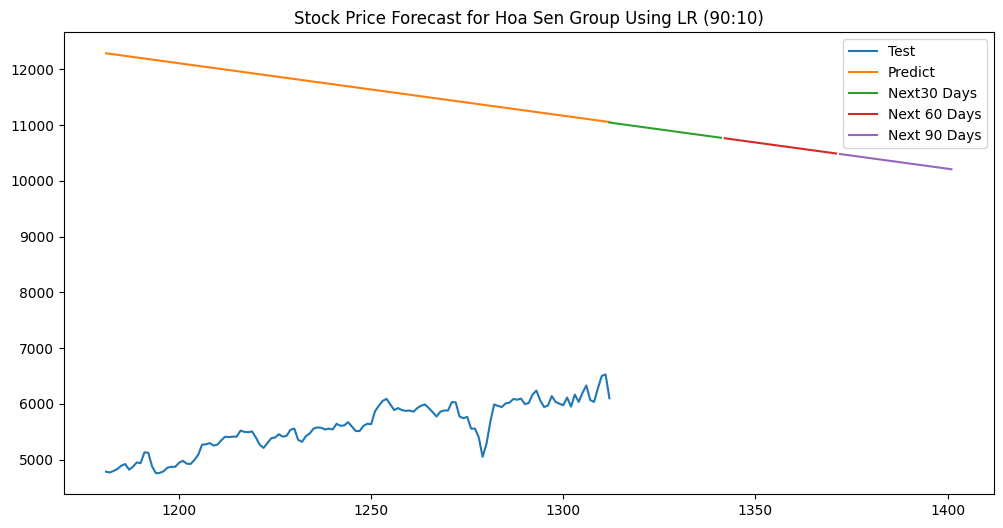
\includegraphics[width=\linewidth]{bibliography/LN_HSG_90-10.png}
    \caption{Linear Regression model's result with 9:1 splitting proportion}
    \label{fig15}
  \end{minipage}
\end{figure}
\begin{figure}[H]
  \centering
  \begin{minipage}{0.8\linewidth}
    \centering
    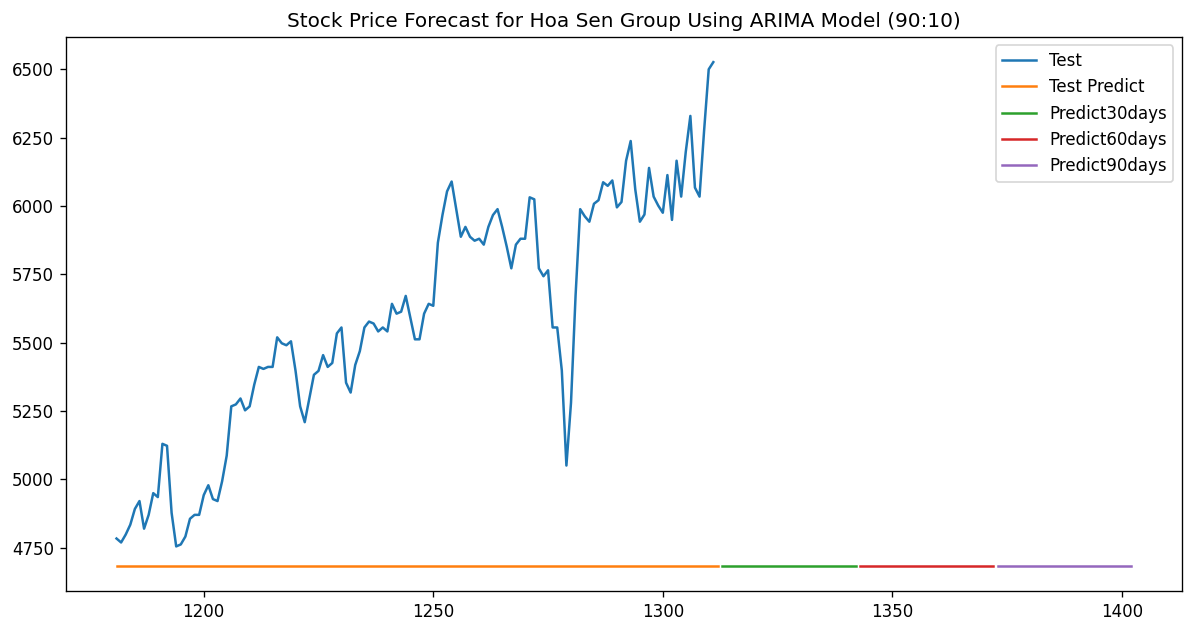
\includegraphics[width=\linewidth]{bibliography/ARIMA_HSG_90-10.png}
    \caption{ARIMA model's result with 9:1 splitting proportion}
    \label{fig16}
  \end{minipage}
\end{figure}
\begin{figure}[H]
  \centering
  \begin{minipage}{0.8\linewidth}
    \centering
    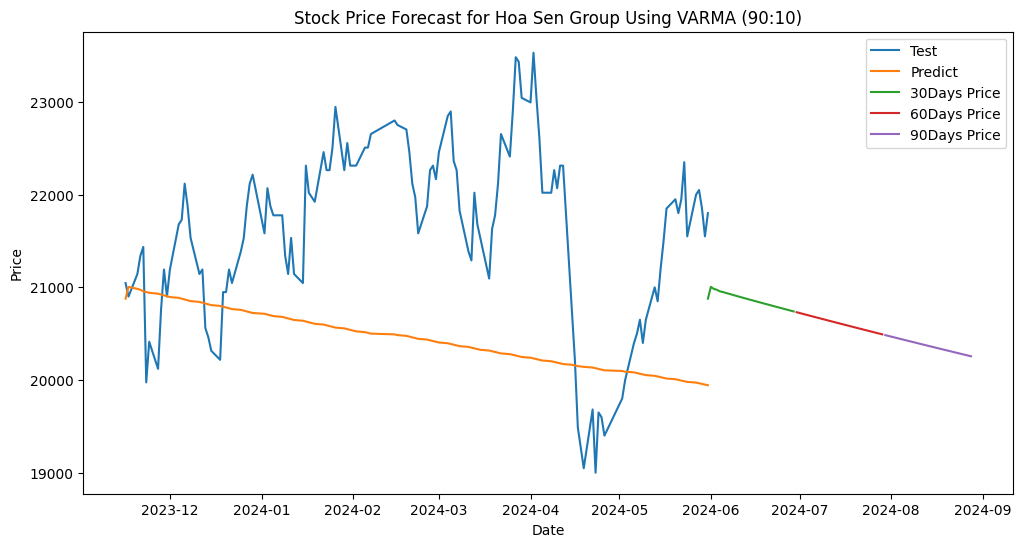
\includegraphics[width=\linewidth]{bibliography/VARMA_HSG_90-10.png}
    \caption{VARMA model's result with 9:1 splitting proportion}
    \label{fig17}
  \end{minipage}
\end{figure}
\begin{figure}[H]
  \centering
  \begin{minipage}{0.8\linewidth}
    \centering
    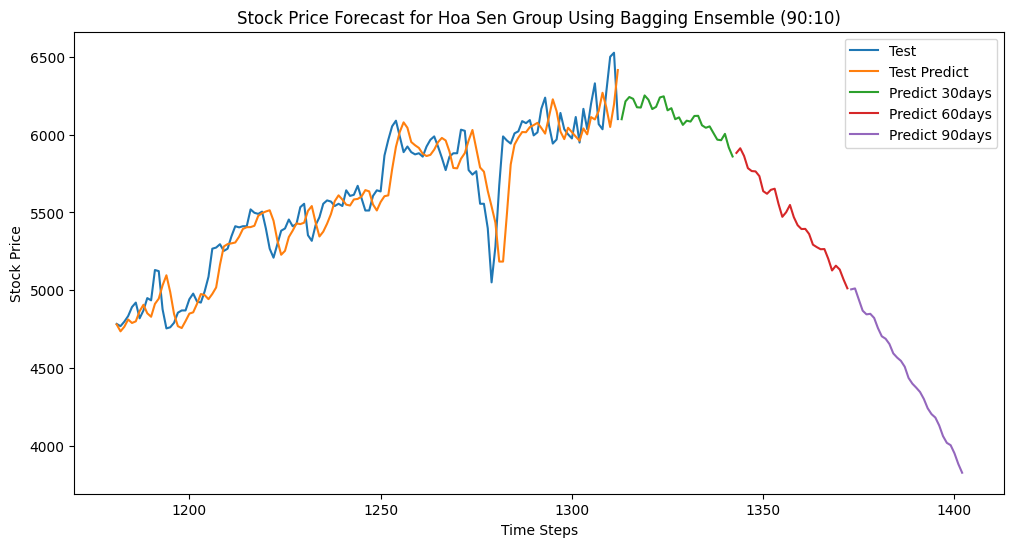
\includegraphics[width=\linewidth]{bibliography/Bagging_HSG.png}
    \caption{BaggingRNN-GRU model's result with 9:1 splitting proportion}
    \label{fig18}
  \end{minipage}
\end{figure}
\begin{figure}[H]
  \centering
  \begin{minipage}{0.8\linewidth}
    \centering
    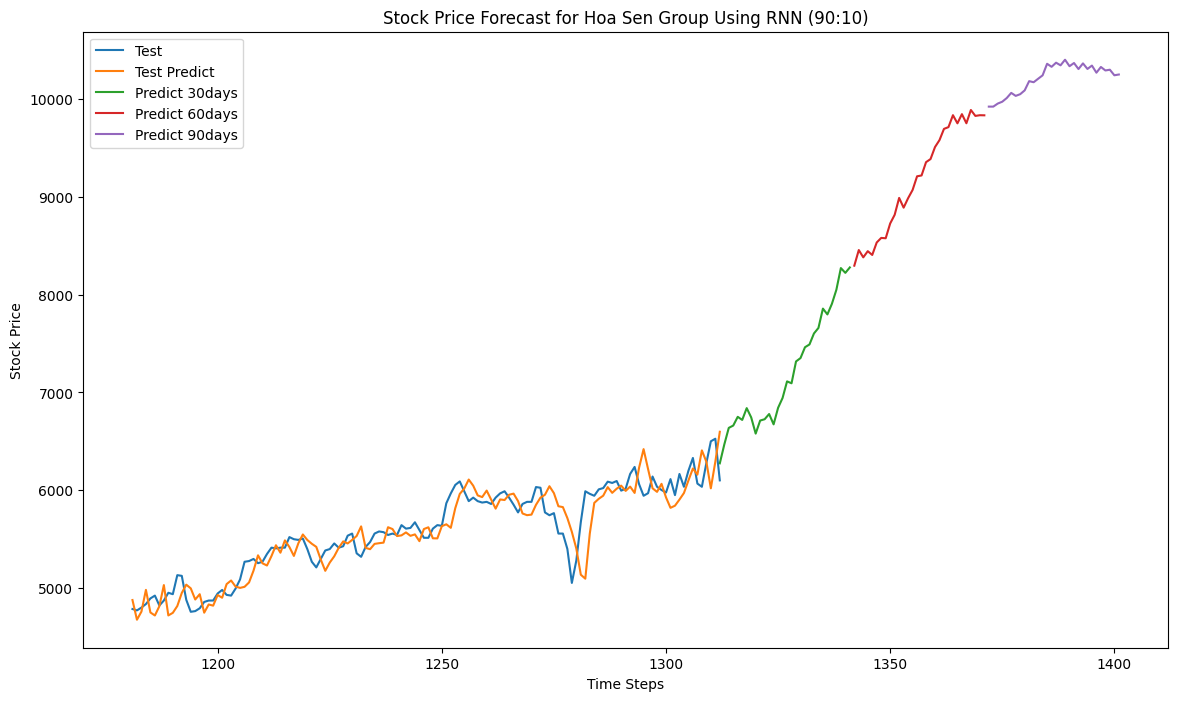
\includegraphics[width=\linewidth]{bibliography/RNN_HSG.png}
    \caption{RNN model's result with 9:1 splitting proportion}
    \label{fig19}
  \end{minipage}
\end{figure}
\begin{figure}[H]
  \centering
  \begin{minipage}{0.8\linewidth}
    \centering
    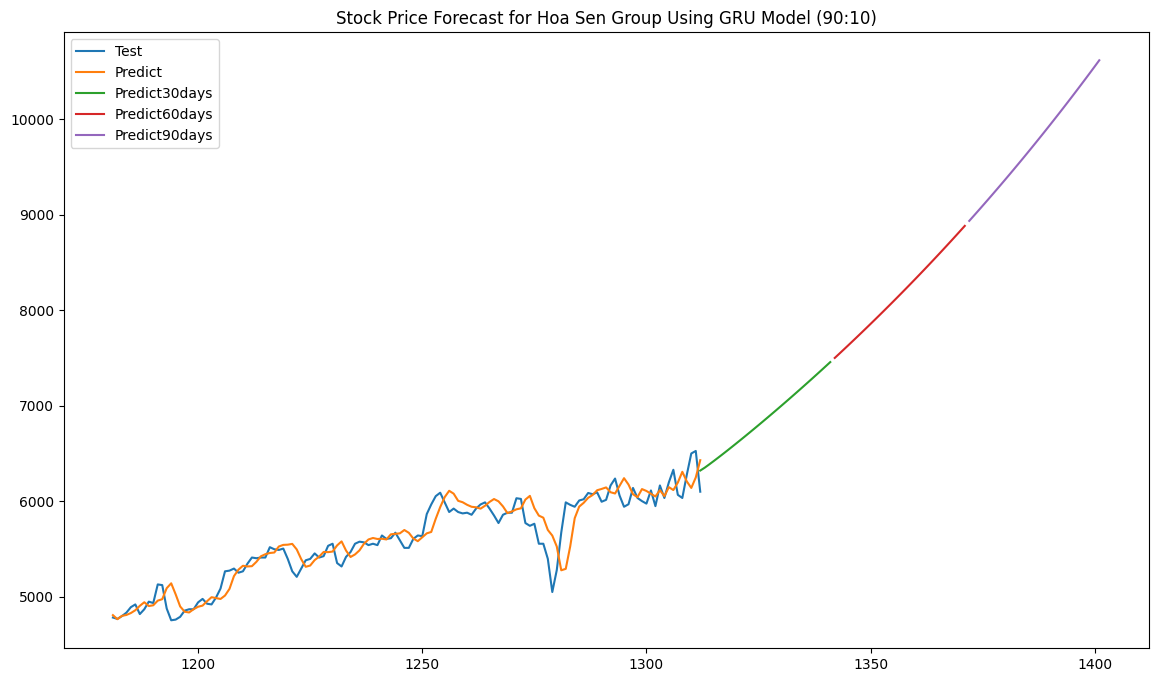
\includegraphics[width=\linewidth]{bibliography/GRU_HSG_90-10.png}
    \caption{GRU model's result with 9:1 splitting proportion}
    \label{fig20}
  \end{minipage}
\end{figure}
\begin{figure}[H]
  \centering
  \begin{minipage}{0.8\linewidth}
    \centering
    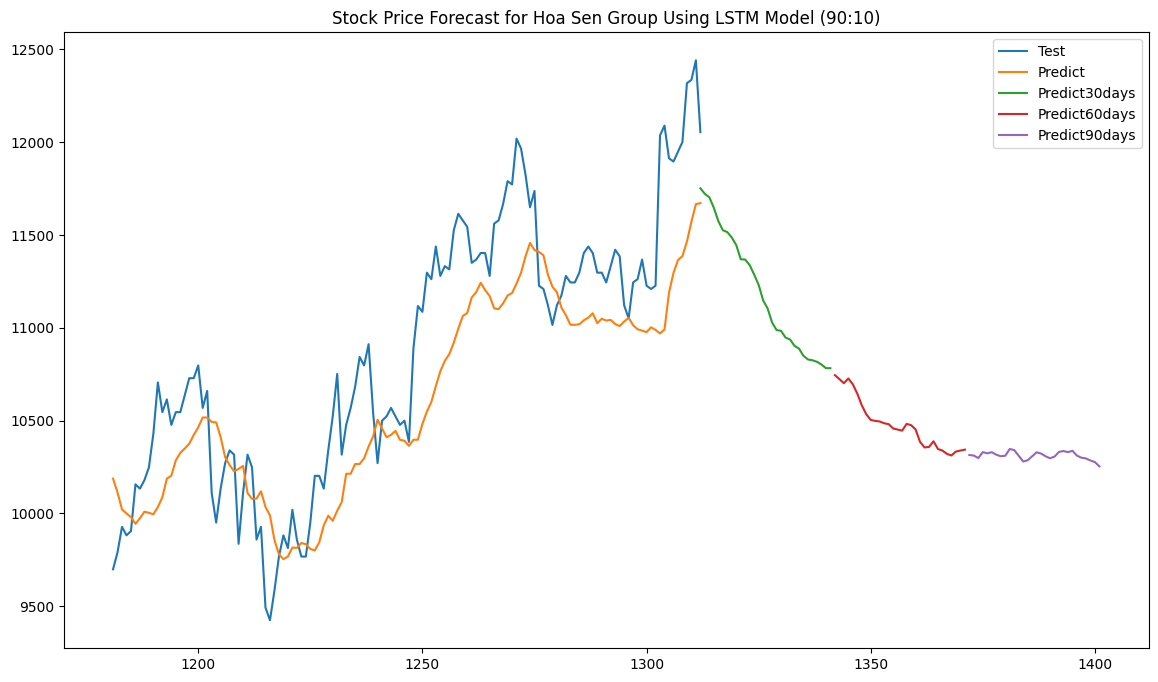
\includegraphics[width=\linewidth]{bibliography/LSTM_HSG_90-10.png}
    \caption{LSTM model's result with 9:1 splitting proportion}
    \label{fig21}
  \end{minipage}
\end{figure}
\begin{figure}[H]
  \centering
  \begin{minipage}{0.8\linewidth}
    \centering
    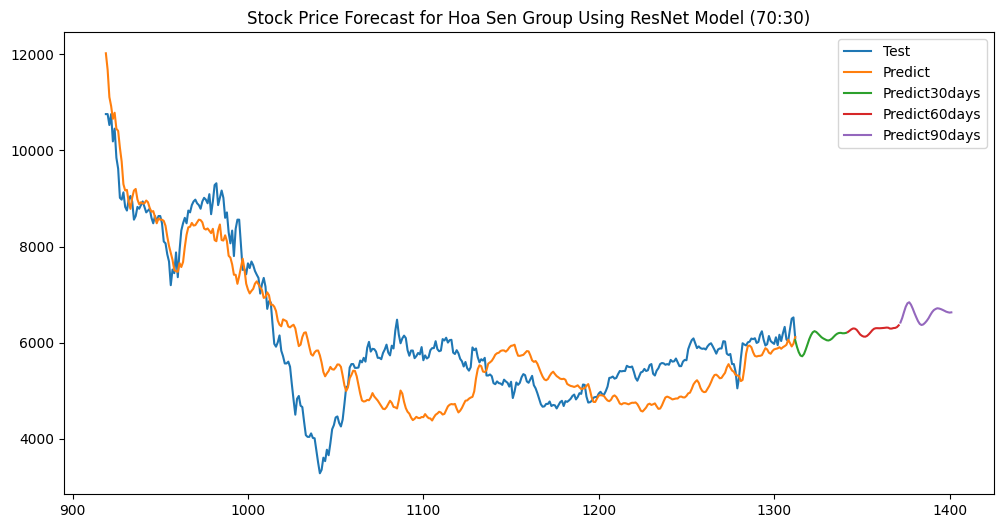
\includegraphics[width=\linewidth]{bibliography/ResNet_HSG_70-30.png}
    \caption{ResNet model's result with 7:3 splitting proportion}
    \label{mbbbggg}
  \end{minipage}
\end{figure}
Given that the models performed better on the 90/10 data split, the three best-performing models are RNN, GRU, and BaggingRNN-GRU. However, the 30, 60, and 90-day predictions for RNN and GRU show an upward trend, while BaggingRNN-GRU predicts a downward trend. This highlights the inherent uncertainty of stock price forecasting
\subsection{NKG dataset} 
\begin{table}[H]
    \centering
    \begin{tabular}{|c|c|c|c|c|}
         \hline
         \multicolumn{5}{|c|}{\textbf{NKG Dataset's Evaluation}}\\
         \hline
         \centering Model & Training:Testing & RMSE & MAPE (\%) & MAE\\
         \hline
         \multirow{2}{*}{LN} & 7:3 & 14261.51 & 327.09 & 14247.65 \\ & 8:2 & 6321.35 & 144.61 & 6247.94 \\ & \textbf{9:1} & \textbf{2643.43} & \textbf{59.49} & \textbf{2484.39}\\
         \hline
         \multirow{2}{*}{ARIMA} & 7:3&1155.03&24.91&1019.82\\ & 8:2&2008.31&40.93&1827.73 \\ & \textbf{9:1} & \textbf{622.55} & \textbf{11.48} & \textbf{515.72}\\
         \hline
         \multirow{2}{*}{VARMA} & 7:3	& 6645.97 &  0.27 & 5457.52 \\ & 8:2 & 7100.67 & 0.28 & 6290.94 \\ & \textbf{9:1} & \textbf{3565.43}  & \textbf{0.14} & \textbf{3331.86}\\
         \hline
         \multirow{2}{*}{Bagging} & 7:3 &  136.825 &  2.140 & 96.220 \\ & 8:2 &  130.649 & 1.912 & 87.971 \\{RNN-GRU} & \textbf{9:1} & \textbf{88.032}  & \textbf{1.454} & \textbf{63.741}\\
         \hline
         \multirow{2}{*}{RNN} & 7:3	& 192.812 & 3.473 & 153.628 \\ & \textbf{8:2} & \textbf{115.154} & \textbf{1.784} & \textbf{82.086} \\ & 9:1 & 116.064 & 1.999 & 86.353\\
         \hline
         \multirow{2}{*}{GRU} & 7:3 & 202.52 & 3.85 & 170.91 \\  & 8:2 &131.21	&1.78&82.65 \\ & \textbf{9:1} & \textbf{95.73} & \textbf{1.64} & \textbf{71.85} \\
         \hline
         \multirow{2}{*}{LSTM} & 7:3 & 913.347 & 20.494 & 859.441 \\ & 8:2 & 329.470 &4.902 & 234.700 \\ & \textbf{9:1} &  	\textbf{207.719} &	\textbf{3.404} & 	\textbf{154.192} \\
         \hline
         \multirow{2}{*}{ResNet} & 7:3 & 1138.96 &  22.49 &  1035.09 \\ & \textbf{8:2} & \textbf{625.87} & \textbf{11.38} & \textbf{486.38}\\ & 9:1 & 848.29 &  19.79 &  835.3 \\ 
         \hline
    \end{tabular}
    \caption{NKG Dataset's Evaluation}
    \label{mbbresult}
\end{table}

For the NKG Stock dataset, most models still achieve the highest performance according to the metric in the 90/10 data split. In particular, for RNN, the best result is obtained on the 80/20 test set, but the result on 90/10 is also good, indicating that the model is quite compatible with the data. Notably, with ResNet, the best evaluation result is obtained on the balanced training and test data of 80/20.
\begin{figure}[H]
  \centering
  \begin{minipage}{0.8\linewidth}
    \centering
    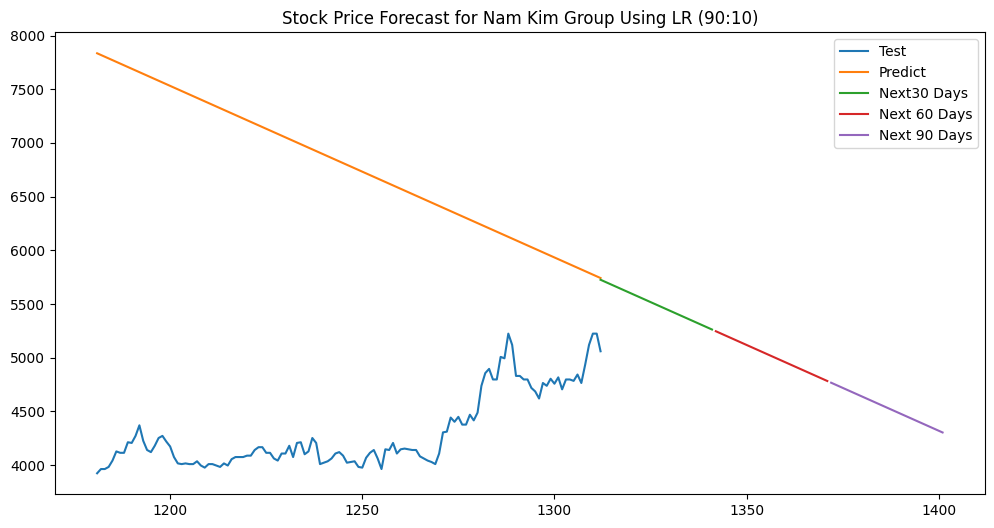
\includegraphics[width=\linewidth]{bibliography/LN_NKG_90-10.png}
    \caption{Linear Regression model's result with 9:1 splitting proportion}
    \label{fig22}
  \end{minipage}
\end{figure}
\begin{figure}[H]
  \centering
  \begin{minipage}{0.8\linewidth}
    \centering
    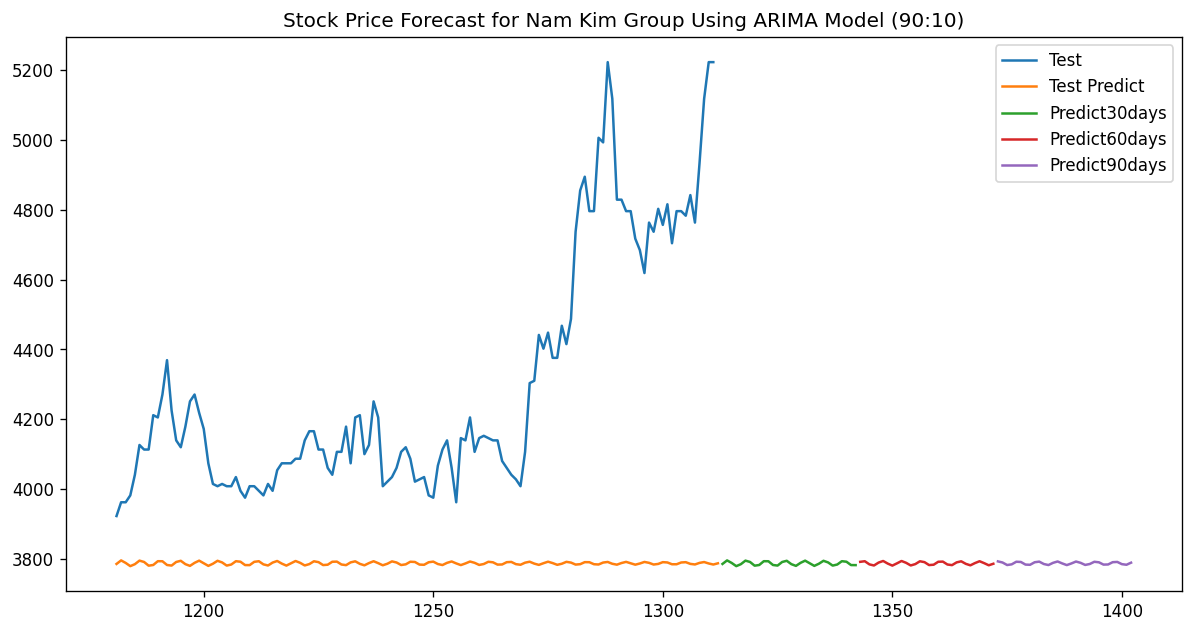
\includegraphics[width=\linewidth]{bibliography/ARIMA_NKG_90-10.png}
    \caption{ARIMA model's result with 9:1 splitting proportion}
    \label{fig23}
  \end{minipage}
\end{figure}
\begin{figure}[H]
  \centering
  \begin{minipage}{0.8\linewidth}
    \centering
    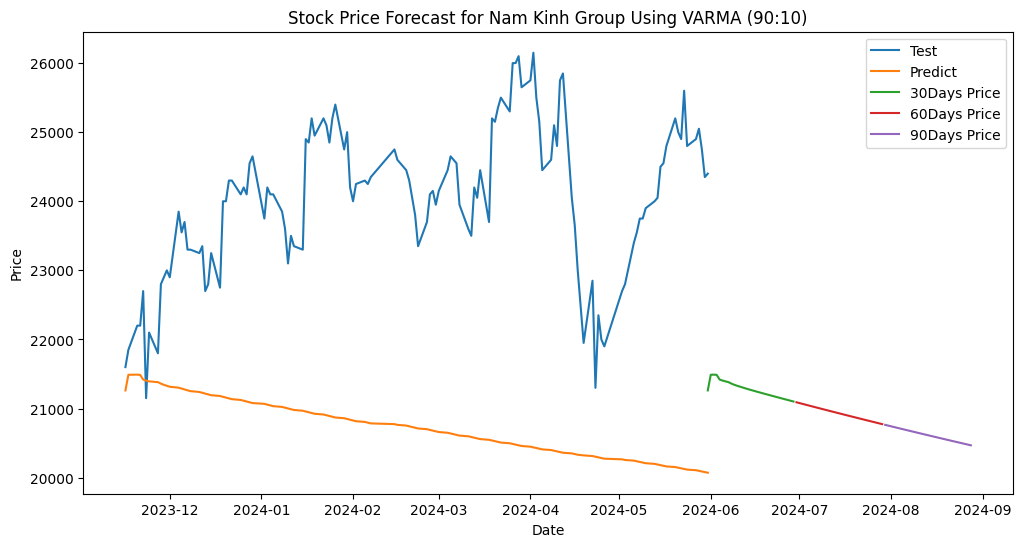
\includegraphics[width=\linewidth]{bibliography/VARMA_NKG_90-10.png}
    \caption{VARMA model's result with 9:1 splitting proportion}
    \label{fig24}
  \end{minipage}
\end{figure}
\begin{figure}[H]
  \centering
  \begin{minipage}{0.8\linewidth}
    \centering
    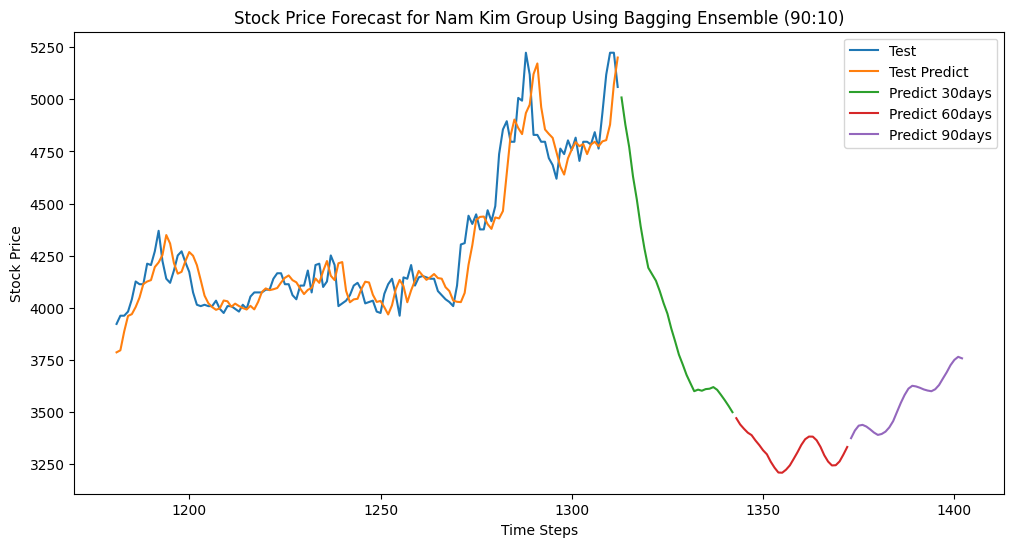
\includegraphics[width=\linewidth]{bibliography/Bagging_NKG.png}
    \caption{BaggingRNN-GRU model's result with 9:1 splitting proportion}
    \label{fig25}
  \end{minipage}
\end{figure}
\begin{figure}[H]
  \centering
  \begin{minipage}{0.8\linewidth}
    \centering
    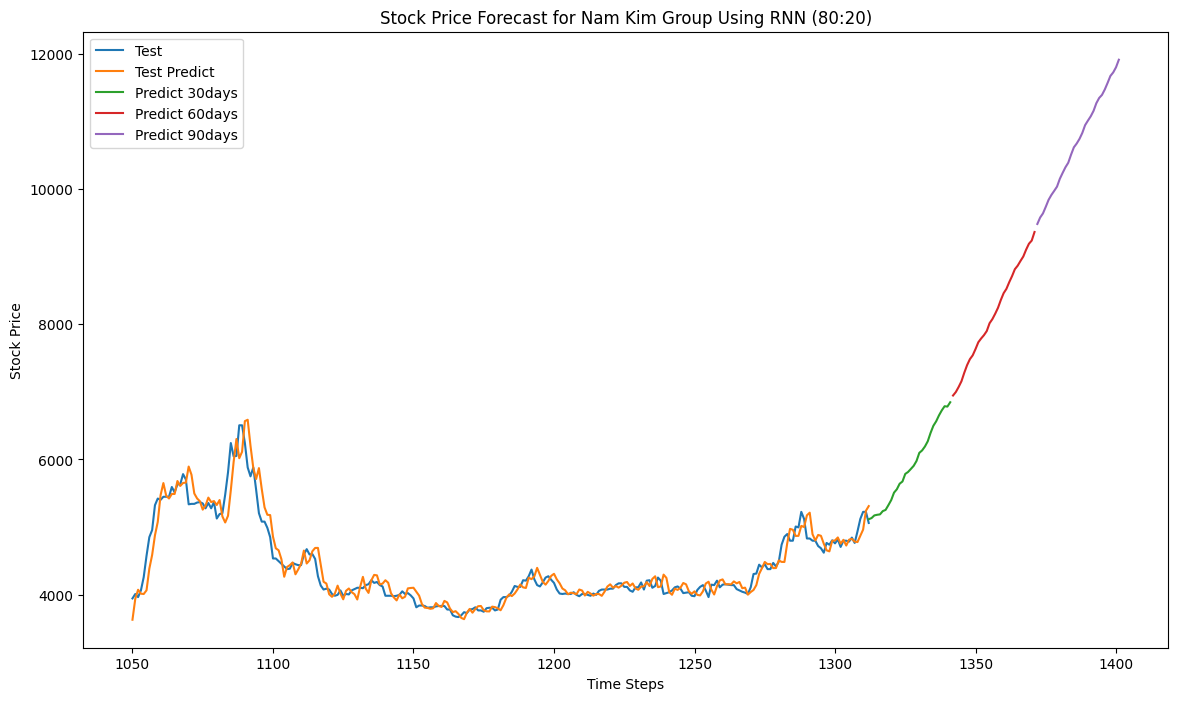
\includegraphics[width=\linewidth]{bibliography/RNN_NKG.png}
    \caption{RNN model's result with 8:2 splitting proportion}
    \label{fig26}
  \end{minipage}
\end{figure}
\begin{figure}[H]
  \centering
  \begin{minipage}{0.8\linewidth}
    \centering
        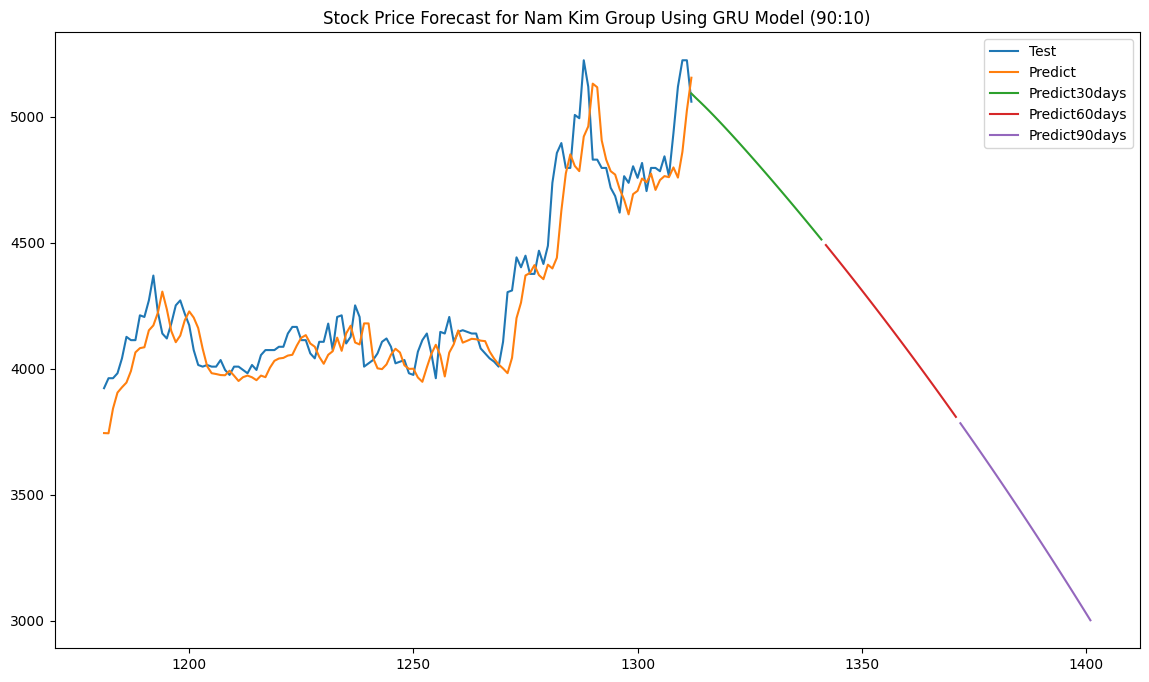
\includegraphics[width=\linewidth]{bibliography/GRU_NKG_90-10.png}
    \caption{GRU model's result with 9:1 splitting proportion}
    \label{fig27}
  \end{minipage}
\end{figure}
\begin{figure}[H]
  \centering
  \begin{minipage}{0.8\linewidth}
    \centering
        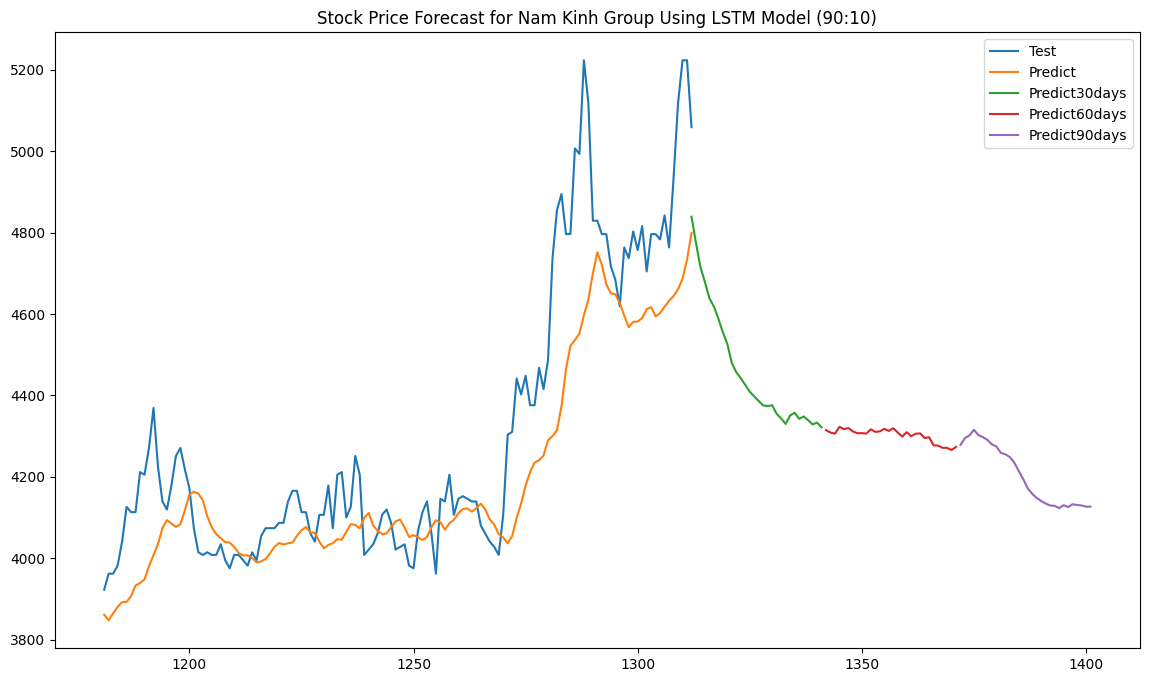
\includegraphics[width=\linewidth]{bibliography/LSTM_NKG_90-10.png}
    \caption{LSTM model's result with 9:1 splitting proportion}
    \label{fig28}
  \end{minipage}
\end{figure}
\begin{figure}[H]
  \centering
  \begin{minipage}{0.8\linewidth}
    \centering
        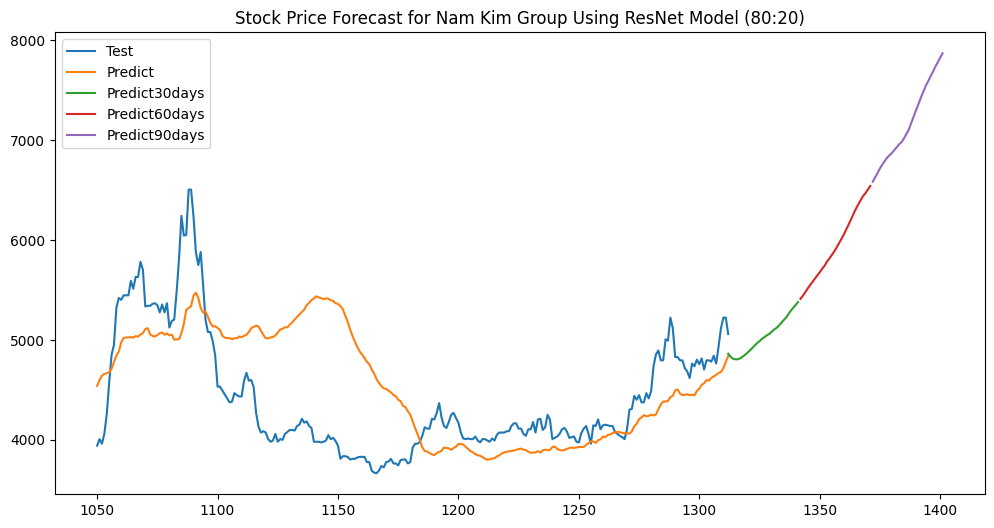
\includegraphics[width=\linewidth]{bibliography/ResNet_NKG_80-20.png}
    \caption{ResNet model's result with 8:2 splitting proportion}
    \label{fig28}
  \end{minipage}
\end{figure}
In the experiments with the best-performing models, during the 30-60-90 day prediction, GRU showed a decreasing trend in the results, while RNN showed an increasing trend. For this dataset, BaggingRNN-GRU showed an uneven fluctuation in the results due to the packaging of the two aforementioned models. The prediction results of the ResNet model with the 80-20 phase also showed a decreasing trend.
\section{Conclusion}
\subsection{Summary}
Steel stock price prediction has gained increasing attention due to the industry's stability and security, making it a sustainable investment. However, stock prices are notoriously difficult to predict due to various external factors. Our research focuses on evaluating algorithms for time series data prediction. Experiments show that RNN, GRU, and BaggingRNN-GRU are the best-performing models based on MAE, MAPE, and RMSE metrics. However, predicting future data through 30-60-90 day forecasts can only identify future trends in the time series, not specific values. The study's findings can aid data analysts in evaluating and predicting short-term time series data.
\subsection{Challenges Encountered}
During the development and implementation of our predictive models "\textbf{Investigating the Efficacy of Statistical, Machine Learning, and Deep Learning
Approaches in Steel Stock Price Prediction}", several challenges were encountered that impacted the progress and outcomes of the project. Here are the key challenges:\\
\indent\textbullet\ \textbf {Model Complexity and Computational Resources}:
Implementing advanced machine learning models, such as BaggingRNN-GRU and Varma, involved dealing with high computational complexity. The training process for fine-tuning hyperparameters significantly increased the computational burden, requiring significant time and resources to achieve optimal performance.\\
\indent\textbullet\ \textbf{Parameter Optimization}:
Identifying the best set of parameters for each model was a non-trivial task. The parameter space for models like ARIMA and RNN is vast and further compounded by the need to balance model complexity with overfitting and underfitting concerns.
\subsection{Future Considerations}
The future research plans focus on improving the existing models for stock price prediction:\\
\indent\textbullet\ \textbf{Increase accuracy}: The main goal is to make the models more precise in their forecasts. This includes understanding the models' parameters and how to combine them for better performance.\\
\indent\textbullet\ \textbf{Continuous improvement}: By incorporating new features, data sources, and advanced techniques, the research aims to constantly refine the models for reliable stock price predictions.
\section*{Acknowledgment}
\addcontentsline{toc}{section}{Acknowledgment}
We are deeply indebted to our esteemed lecturer \textbf{Assoc. Prof. Dr. Nguyen Dinh Thuan}, and instructors \textbf{TA. Trinh Thi Thanh Truc} and \textbf{TA. Dang Vu Phuong Uyen}, for their exceptional guidance and unwavering support throughout this research journey. Their expertise and insightful feedback were instrumental in shaping the direction and refining the quality of our study, helping our group gain a clearer understanding of the research problem.

%% UNCOMMENT these lines below (and remove the 2 commands above) if you want to embed the bibliografy.
\begin{thebibliography}{100}

\bibitem{b1} E. R. Warsono, Wamiliana, Widiarti, and M. Usman, ''Modeling and forecasting by the vector autoregressive moving average model for export of coal and oil data (case study from Indonesia over the years 2002-2017),'' June 2019. [Online]. Available: doi.org/10.32479/ijeep.7605.

\bibitem{b2} Umut Ugurlu, Ilkay Oksuz and Oktay Tas, "Electricity Price Forecasting Using Recurrent," MDPI, 14 May 2018.

\bibitem{b3} H. Choi, S. Ryu, and H. Kim, ''Short-term load forecasting based on ResNet and LSTM,'' October 2018. [Online]. Available: doi.org/10.1109/SmartGridComm.2018.8587554.

\bibitem{b4} Y.-T. Tsai, Y.-R. Zeng and Y.-S. Chang, "Air Pollution Forecasting Using RNN with LSTM," 2018 October 28. [Online]. Available: https://ieeexplore.ieee.org/document/8512020.

\bibitem{b5} Corporate Finance Institute (CFI), ''Regression analysis,'' [Online]. Available: https://corporatefinanceinstitute.com/resources/data-science/regression-analysis.

\bibitem{b6} Scribbr, ''Multiple linear regression,'' [Online]. Available: https://www.scribbr.com/statistics/multiple-linear-regression.

\bibitem{b7} Penn State University (STAT 462), ''The multiple linear regression model,'' [Online]. Available: https://online.stat.psu.edu/stat462/node/131.

\bibitem{b8}G. Box and G. Jenkins, Time Series Analysis: Forecasting and Control, San Francisco: Holden-Day, 1970. 

\bibitem{b9}M. Zhang, "Time Series: Autoregressive models AR, MA, ARMA, ARIMA," 2018.

\bibitem{b10} K. D. Pham, ''Bài 19 - Mô hình ARIMA trong time series,'' December 2019. [Online]. Available: phamdinhkhanh.github.io/2019/12/12/ARIMAmodel.html. [Accessed April 2024].

\bibitem{b11} Analytics India Magazine (AIM), ''A guide to VARMA with Auto ARIMA in time series modelling,'' [Online]. Available: https://analyticsindiamag.com/a-guide-to-varma-with-grid-search-in-time-series-modelling.

\bibitem{b12} S. Link, "Applied Time Series Analysis and Forecasting with Python," 20 October 2022. [Online]. Available: https://link.springer.com/chapter/10.1007/978-3-031-13584-2-7.

\bibitem{b13} H. Lutkepohl, ''Forecasting with VARMA models,'' [Online]. Available: https://cadmus.eui.eu/bitstream/handle/1814/2805/ECO2004-25.pdf.

\bibitem{b14} Simplilearn, "Bagging in machine learning: Step to perform and its advantages," 13 May 2024. [Online]. Available: https://www.simplilearn.com/tutorials/machine-learning-tutorial/bagging-in-machine-learning.

\bibitem{b15} Y.-T. Tsai, Y.-R. Zeng and Y.-S. Chang, "Air Pollution Forecasting Using RNN with LSTM," 2018 October 28. [Online]. Available: https://ieeexplore.ieee.org/document/8512020.

\bibitem{b16} GeeksforGeeks, "Introduction to recurrent neural network," 4 December 2023. [Online]. Available: https://www.geeksforgeeks.org/introduction-to-recurrent-neural-network.

\bibitem{b17} Geeksforgeeks, "Activation functions in Neural Networks," 3 may 2024. [Online]. Available: https://www.geeksforgeeks.org/activation-functions-neural-networks/.

\bibitem{b18} NVIDIA Developer, ''Long short-term memory (LSTM),'' [Online]. Available: https://developer.nvidia.com/discover/lstm.

\bibitem{b19} Machine Learning Mastery, ''Introduction long short term memory networks experts,'' [Online]. Available: https://machinelearningmastery.com/gentle-introduction-long-short-term-memory-networks-experts.

\bibitem{b20} N. Buslim, I. L. Rahmatullah, and B. A. Setyawan, "Comparing Bitcoin's Prediction Model Using GRU, RNN, and LSTM by Hyperparameter Optimization Grid Search and Random Search," in 2021 9th International Conference on Cyber and IT Service Management (CITSM), pp. 1-5, doi: 10.1109/CITSM53870.2021.00002 (2021).

\bibitem{b21} Z. G. Wang, W. Z. Yan, and T. Oates, ''Time series classification from scratch with deep neural networks: A strong baseline,'' Dec. 2016. [Online]. Available: arxiv.org/pdf/1611.06455.

\bibitem{b22} K. Cho, B. Van Merriënboer, D. Bahdanau, and Y. Bengio, ''On the properties of neural machine translation: encoder-decoder approaches,'' 2014.

\end{thebibliography}
\EOD

\end{document}
